% =============================================================================================
% Predicting the experimental lattice thermal conductivity of half-Heusler compounds
% by machine learning and transfer-function calibration
%
% Target journal: Computational Materials Science (Elsevier), elsarticle class.
%
% TO COMPILE (Overleaf: upload this folder, set manuscript.tex as the main document):
%     pdflatex manuscript  ->  bibtex manuscript  ->  pdflatex x2
%
% BEFORE SUBMITTING, run the gates from the repository root:
%     python audit_completion.py             every table cell and headline number against its artefact
%     python check_tex_structure.py          placeholders, control characters, structure
%     python verify_citations.py paper/manuscript.tex
% The last fails on an undefined citation key, a DOI that no longer resolves, or a citation
% with no recorded supporting sentence in claims_ledger.csv. All are blocking.
%
% Authors, affiliations and all four ORCIDs are set; see the frontmatter comment below.
% =============================================================================================

% `authoryear` puts natbib in author-year mode, which contradicts \bibliographystyle{elsarticle-num}
% below and renders the citations malformed. Every citation in this manuscript is a plain \cite --
% there is no \citep or \citet anywhere -- so the numeric style is the one we want and the class
% option is what has to go.
\documentclass[final,5p,times,twocolumn]{elsarticle}

\usepackage[T1]{fontenc}
\usepackage[utf8]{inputenc}      % author names carry o-slash, s-caron, l-stroke etc.
\usepackage{amsmath, amssymb}
\usepackage{graphicx}
\usepackage{booktabs}
\usepackage[separate-uncertainty=true, detect-weight=true]{siunitx}
\usepackage[version=4]{mhchem}
\usepackage{microtype}
\usepackage{enumitem}            % the numbered contributions list closing the Introduction
\usepackage[hidelinks]{hyperref}

% elsarticle's \corref and \cnotenum end up inside the string hyperref builds for the PDF's
% metadata, which it cannot typeset -- that is the "Token not allowed in a PDF string" warning
% repeated for every author. Supplying the metadata explicitly silences it and, more usefully,
% puts a correct title and author list into the PDF's document properties, which is what indexers
% and reference managers read.
\hypersetup{
  pdftitle  = {Predicting the experimental lattice thermal conductivity of half-Heusler
               compounds by machine learning and transfer-function calibration},
  pdfauthor = {Shivam Randive, Heet Lungaria, Ojaswini Randive, Himanshu Pandey},
  pdfsubject= {Lattice thermal conductivity of half-Heusler thermoelectrics},
  pdfkeywords = {half-Heusler, lattice thermal conductivity, thermoelectric,
                 Boltzmann transport equation, machine learning, transfer-function calibration,
                 experimental validation}}

% Half Heuslers are written as \ce{ZrNiSn}; keep chemistry upright inside bold table cells.
\sisetup{group-separator = {,}, group-minimum-digits = 4}

% =============================================================================================
% WHAT MUST STILL BE FILLED IN BEFORE SUBMISSION.
% Each is rendered into the PDF, so it is defined here rather than left inline where it can be
% missed. check_tex_structure.py fails the build while any of them still says TO BE ADDED.
% =============================================================================================
% Authors and affiliations are complete: Shivam Randive, Heet Lungaria and Himanshu Pandey at
% SVNIT Surat; Ojaswini Randive at NIT Raipur (confirmed 2026-09-18, with ORCID). The department
% given for NIT Raipur is Metallurgical and Materials Engineering -- confirm it is hers.
% The \ead is i22ph019@phy.svnit.ac.in, attached to Shivam Randive as corresponding author.
\newcommand{\pandeyemail}{hp@phy.svnit.ac.in}
% Heet Lungaria's CRediT roles, set to match Ojaswini Randive's on the first author's instruction:
% both contributed to the figures. If the phonon-stability analysis is later added to the paper,
% this line should be revised to name that contribution -- but only once the analysis is actually
% IN the manuscript, since CRediT describes contributions to this work.
\newcommand{\heetroles}{Visualization, Writing -- review \& editing.}
% Zenodo archive of the GitHub repository, minted from release v1.0.0.
% Zenodo issues TWO DOIs: a version DOI pinned to this exact snapshot, and a concept DOI that
% always resolves to the newest version. The version DOI is used here so a referee gets precisely
% the code that produced these numbers. Confirm on the Zenodo record page that 22642666 is the one
% labelled "Version DOI"; if the labels are the other way round, swap the two numbers below.
\newcommand{\repourl}{\href{https://doi.org/10.5281/zenodo.22642666}%
  {\texttt{doi:10.5281/zenodo.22642666}} (concept DOI
  \href{https://doi.org/10.5281/zenodo.22642665}{\texttt{10.5281/zenodo.22642665}}, which resolves
  to the latest version)}
% Draft. Confirm the Google credit programme's exact name before submission -- funders and credit
% schemes usually specify the wording they want to be acknowledged by, and getting it wrong is
% worse than omitting it. Add any departmental or institutional support Prof. Pandey advises.
% Counts: provenance_sources.measurement_source_dois (189) and .calculation_source_dois (29) in
% data/exports/kappa_v2/paper_numbers.json.
% FUNDING STATEMENT: the journal's stock no-funding sentence, chosen by the authors (2026-10-05);
% see the Funding section. The Google Cloud credits are acknowledged below as in-kind support.
\newcommand{\acknowledgementtext}{%
  Google Cloud credits funded the large-language-model extraction of measurements from primary
  publications (Section~\ref{sec:dataset}). We thank the maintainers of the databases this work
  rests on (Starrydata2, AFLOW, the Materials Project, JARVIS, OQMD, DxMag, the Crystallography Open
  Database and the OPTIMADE consortium), whose curation made an experiment-anchored corpus of this
  kind possible. We also thank the authors of the \num{189} experimental and \num{29} computational
  studies whose measurements and calculations make up the corpus analysed here.}

\journal{Computational Materials Science}

\begin{document}

\begin{frontmatter}

\title{Predicting the experimental lattice thermal conductivity of half-Heusler compounds
       by machine learning and transfer-function calibration}

% Author order follows the convention of the field: first author did the work, last author is the
% senior/supervising author, middle authors contributed in between. The last position is the
% SECOND most senior, not the least -- putting the supervisor in the middle of a three-author list
% would place him in the weakest slot and imply the third author supervised the project.
% Confirm this order with Prof. Pandey before submission; some departments prefer otherwise.
% ORCID iDs are supplied to Elsevier through Editorial Manager at submission, not through the
% .tex -- elsarticle has no \orcid macro and the publisher adds the iD badges from the submission
% record. Kept here so they are not lost:
%   Shivam Randive    0009-0005-1403-4484   (checksum verified)
%   Heet Lungaria     0009-0007-5249-6764   (checksum verified)
%   Ojaswini Randive  0009-0003-3210-8120   (checksum verified)
%   Himanshu Pandey   0000-0002-7380-366X   (checksum verified)
\author[svnit]{Shivam Randive\corref{cor1}}
\ead{i22ph019@phy.svnit.ac.in}
\author[svnit]{Heet Lungaria}
\author[nitrr]{Ojaswini Randive}
\author[svnit]{Himanshu Pandey\corref{cor1}}
\ead{\pandeyemail}
\cortext[cor1]{Corresponding authors.}

\affiliation[svnit]{organization={Department of Physics, Sardar Vallabhbhai National Institute
                                  of Technology},
                    city={Surat},
                    country={India}}
% Confirm the department's exact official name against the NIT Raipur website before submission:
% affiliations are indexed verbatim by Scopus and Web of Science, so a paraphrase can detach the
% paper from the institution's record.
\affiliation[nitrr]{organization={Department of Metallurgical and Materials Engineering,
                                  National Institute of Technology Raipur},
                    city={Raipur},
                    state={Chhattisgarh},
                    country={India}}

% =============================================================================================
% ABSTRACT + KEYWORDS.
%
% Every number here is quoted from data/exports/kappa_v2/paper_numbers.json; none is typed by hand.
%   1.69, 34, 10 of 12           offset.median_ratio_calc_over_meas / n_compounds /
%                                families_with_median_ratio_above_1 of n_families
%   21.9                         ml_generator_validation.median_ape (single seed)
%   33.1, 87.2, 39, five seeds   in_domain_table.seed_medians.calibrated (median over seeds), .n
%   41.9                         in_domain_table.seed_medians.uncorrected_surrogate.median_ape.median
%   46.7, 45.6                   in_domain_table.nulls.constant / .power .median_ape
%   0.004                        in_domain_table.paired_p_seed_median (both nulls; paired Wilcoxon)
%   18, 0.048                    cluster_level_significance n_clusters, wilcoxon_p_max (power,
%                                0.0483, so "p < 0.05 on every seed, largest 0.048")
%   38.6, 78.9, 50               headline.unconditional; blind_test.compounds
%   32.3, 31                     deployed_route.held_out.global_on_same_compounds.median_ape, .n
%   21.7                         deployed_route.held_out.median_ape
%   5 families, 7.4-24.9         family_calibration.n_validated_under_25; min/max of
%                                adopted.*.loo_family_ape over families under 25
%   10 issued, 15 flagged        predictions.counts (ISSUED, FLAGGED)
%
% Length: <= 250 words of rendered text (Computational Materials Science). Started from
% Alternative A of paper/review/clarity_front_back_supp.md; 249 words counted with wc -w on the
% rendered text (each formula token counted as typeset).
% Shape: the gap (models reproduce calculations), the offset that makes a correction necessary,
% the two steps, the end-to-end headline with its scope and the nulls, the comparison with
% calibrating a published calculation, the family constants, predictions. The two separately
% validated errors of a structure-only value are stated side by side in the body and never merged.
% audit_completion.py checks that 33.1 and 87.2 appear here as \SI{..}{\percent}.
% =============================================================================================

\begin{abstract}
Predicting the measured lattice thermal conductivity ($\kappa_L$) of half-Heusler thermoelectrics
is hard: first-principles Boltzmann-transport-equation (BTE) calculations, and machine-learned
models trained on them, reproduce calculations, not measurements.
Published calculations exceed measured half-Heusler $\kappa_L$ by a median factor of \num{1.69}
(\num{34} compounds; \num{10} of \num{12} bonding families). A machine-learned model predicts the BTE value from crystal structure (median error
\SI{21.9}{\percent} against published calculations, single seed). A closed-form transfer function,
$\kappa_L^{\mathrm{exp}} = \kappa_L^{\mathrm{BTE}}\min[c\,(T/300)^p, 1]$, fitted on published
calculations against one reference laboratory per compound, maps it onto the experimental scale.
Holding each compound's chemistry cluster out of both steps, inside a predefined domain (18
valence electrons, cubic $C1_b$, no known polymorph), the median error is \SI{33.1}{\percent} and \SI{87.2}{\percent} of
\num{39} compounds lie within a factor of two (five-seed median), against \SI{41.9}{\percent}
uncorrected and \SI{46.7}{\percent} and \SI{45.6}{\percent} for constant and power-law baselines
(paired Wilcoxon $p = \num{0.004}$; counting each of \num{18} clusters once, $p < 0.05$ on every
seed, largest \num{0.048}). Unscreened, all \num{50} measured compounds give \SI{38.6}{\percent} and
\SI{78.9}{\percent}. Calibrating published calculations gives a comparable \SI{32.3}{\percent} on a
different set of \num{31} held-out compounds. Per-family constants lower this to
\SI{21.7}{\percent} (not significant compound by compound), and are validated held out, at
\SIrange{7.4}{24.9}{\percent}, in \num{5} bonding families. We issue \num{10} predictions with
intervals, flag \num{15} with reasons, and predict \ce{TmPbAu} and \ce{HfTeOs}, for which we find no
published report, from structure alone.
\end{abstract}

% Keywords: 1-7 allowed (live Guide for Authors); 7 used. Specific terms, no plurals, no "and"/"of".
% Keep pdfkeywords in manuscript.tex identical.
\begin{keyword}
half-Heusler \sep lattice thermal conductivity \sep thermoelectric \sep
Boltzmann transport equation \sep machine learning \sep transfer-function calibration \sep
experimental validation
\end{keyword}


\end{frontmatter}

% =============================================================================================
% SECTION 1 -- INTRODUCTION.
%
% Order: why the property matters; the computational route and its cost; calculation vs
% measurement, ending on the gap; our evidence that the gap matters; prior routes across it and
% what is different here; the scarcity that makes it hard; what this paper does, with the
% definitions a reader needs; the contributions. Condensed 2026-10-05 (research-paper pass).
%
% Every citation is resolved through Crossref and carries a row in claims_ledger.csv with the
% sentence from the source that supports it. None was written from memory.
%
% Numbers from data/exports/kappa_v2/paper_numbers.json:
%   1.69 / 34 / 29 of 34 / 10 of 12   offset.*
%   21, 2.01                      vs_published_model.n_common, .positive_control.sdnnff_vs_measurement
%   18, 0.99                      .positive_control.sdnnff_vs_published_bte_calculation (n, median_ratio)
%   735, 284, 50                  corpus.half_heuslers / half_with_dft_tier1 / half_measured_tier0
%   0.42 / 0.70                   calibration.c / .p
%   5 of 9                        family_calibration.n_validated_under_25 / n_validated
%   21.7 vs 32.3 on 31            deployed_route.held_out (.median_ape, .global_on_same_compounds)
%   0.44                          deployed_route.held_out.sign_test_p_family_vs_shared (0.442)
%   33.0                          shared_constant_unseen_family.median_ape
%   21.9 / 88.3 / 230             ml_generator_validation (single seed)
%   45 descriptors; four regressors   shap_ranking.n_descriptors; model_comparison (4 entries)
%   33.1 / 87.2 / 39              in_domain_table.seed_medians.calibrated, .n
%   41.9                          in_domain_table.seed_medians.uncorrected_surrogate
%   46.7 / 45.6 / 0.004           in_domain_table.nulls, .paired_p_seed_median
%   18 / 0.048                    cluster_level_significance (n_clusters, wilcoxon_p_max.power =
%                                 0.0483); sign_p_range (not significant on every seed)
%   38.6 / 78.9 / 50              headline.unconditional, blind_test.compounds
%   10 / 3 at 500 K / 15          predictions.counts, predictions.issued_quoted_at_500K
%   10 conditional                conditional.n
% =============================================================================================

\section{Introduction}
\label{sec:intro}

A thermoelectric generator needs a material that conducts charge freely but obstructs heat. Half
Heuslers meet the first requirement far better than the second. Their electronic performance is
established, with figures of merit approaching $zT \approx 1.5$ in $p$-type
\ce{FeNbSb}~\cite{fu2015realizing} and $zT \approx 1.4$ in \ce{ZrCoBi}~\cite{zhu2018discovery}, and
the class is mechanically robust, stable to high temperature and made of abundant elements. Their
lattice thermal conductivity $\kappa_L$, however, remains high, and because $zT$ varies inversely
with $\kappa_L$, most advances have come from suppressing it after synthesis. The screening problem
is to identify compounds with intrinsically low $\kappa_L$ before they are made.

Solving the phonon Boltzmann transport equation (BTE) from first principles gives $\kappa_L$ with no
experimental input, and reproduces the measured temperature dependence of a half Heusler without
being fitted to it~\cite{shiomi2011thermal}. The obstacle is cost. Carrete \emph{et al.} calculated
\num{32} half Heuslers in full and trained a random-forest model on them to search a far larger
set~\cite{carrete2014finding}, and much later work has reproduced the calculation more cheaply,
through compressed-sensing descriptors~\cite{liu2020a} and machine-learned models trained on
databases of computed
conductivities~\cite{luo2023predicting,trans2022lattice,miyazaki2021machine,jaafreh2021lattice,bhattacharjee2022thorough}.
The most recent, by Paliwal and Alam, trains an ensemble of seven tree-based regressors on
\num{4127} calculated values for \num{150} compounds and reports $R^2 = \num{0.9994}$ on held-out
calculated labels~\cite{paliwal2025accelerate}.

Such models, which we call \emph{surrogates} because they stand in for the calculation, are
accurate against the quantity they were trained on, and that quantity is a calculation, not a
measurement. The field's assessment of the difference has changed. A 2019 review concluded that
first-principles transport ``agree[s] with experimental measurements for diverse crystalline
materials''~\cite{mcgaughey2019phonon}; a controlled multi-code comparison in 2025, by the same
lead author, found the solvers within \SI{15}{\percent} of their mean values, yet reported that the
calculated conductivities ``do not generally show agreement with experimental
measurements''~\cite{mcgaughey2025phonon}. Paliwal and Alam note that computed $\kappa_L$ ``often
overestimates the experimental values because real samples inevitably contain impurities, defects,
and grain boundaries''~\cite{paliwal2025accelerate}, but treat it as context rather than as a
quantity to measure. What has been missing is the magnitude and sign of the disagreement across a
materials class, and a correction for it validated against held-out experiment.

In our corpus, published transport calculations exceed the measured $\kappa_L$ of the same compound
by a median factor of \num{1.69} over \num{34} compounds. A surrogate that reproduces the calculation
therefore carries that offset when its output is read as a prediction of experiment. A published
neural-network force field, Elemental-SDNNFF~\cite{rodriguez2023millionsca}, shows this
(Section~\ref{sec:sdnnff}): on the \num{21} in-domain compounds it shares with our validation set,
its values are a median \num{2.01} times the measurements, while on the \num{18} that carry a
published calculation they are a median \num{0.99} times that calculation.

Existing routes across this gap do not correct a full BTE calculation. Zhu \emph{et al.}
transfer-learned a crystal-graph network from \num{2668} computed conductivities onto \num{132}
measured values, starting from semi-empirical high-throughput estimates~\cite{zhu2021charting};
Miller \emph{et al.} fitted a semi-empirical model to experiment~\cite{miller2017capturing}; Chen
\emph{et al.} trained a Gaussian process on about one hundred measured solids~\cite{chen2019machine};
and a related study merged empirical estimates, calculations and measurements into one training
target~\cite{liu2022leveraging}. Keeping experiment and calculation apart is what makes the offset
measurable. Our correction acts on the transport calculation itself and is closed-form: a magnitude
and an exponent that can be applied by hand.

Measurements to correct against are scarce. Of the \num{735} half Heuslers in our corpus with any
thermal-conductivity record, \num{284} have a full first-principles transport calculation and
\num{50} have been measured. Training directly on measurements is beginning to
appear~\cite{barua2024interpreta}, but \num{50} compounds are too few to learn a structure--property
relation from scratch. As we show, they are enough to calibrate one.

We predict the measured $\kappa_L$ with two steps used as a pair: a machine-learned model, trained on
full first-principles calculations, predicts the calculation from crystal structure, and a transfer
function maps a calculation onto the experimental scale. Measurements and calculations are never
pooled, and each measured compound is scored against one reference laboratory chosen by a fixed rule
that never reads a calculation. Writing a half Heusler as XYZ (Section~\ref{sec:method}), a
\emph{bonding family} shares its Y and Z elements and a \emph{chemistry cluster} its X element. The
end-to-end test holds each compound's chemistry cluster out of both steps and is compared with
\emph{null baselines} that use no compound-specific information.

Our contributions are:
%
\begin{enumerate}[label=(\roman*), itemsep=1pt, topsep=3pt, leftmargin=2.2em]
  \item A machine-learned model, trained only on full first-principles calculations, that predicts
        $\kappa_L^{\mathrm{BTE}}$ from crystal structure with \num{45} descriptors, selected among
        four regressors trained on identical rows and folds. With each chemistry cluster held out,
        it reproduces published calculations to a median error of \SI{21.9}{\percent} (one seed),
        with \SI{88.3}{\percent} of \num{230} compounds within a factor of two, and its
        \textsc{shap} attribution is consistent with phonon physics.
  \item A closed-form transfer function, $\kappa_L^{\mathrm{exp}} = \kappa_L^{\mathrm{BTE}}
        \min[c\,(T/300)^p, 1]$, that corrects an offset regular across the class: calculations run
        high in \num{29} of \num{34} compounds and in \num{10} of \num{12} bonding families. Fitted
        on published calculations, its shared magnitude $c = \num{0.42}$ is well determined and its
        exponent $p = \num{0.70}$ much less so. On families never measured it gives a median error of
        \SI{33.0}{\percent}. A magnitude refitted per bonding family gives \SI{21.7}{\percent} on
        compounds held out of their own family's fit, against \SI{32.3}{\percent} for the shared
        constant on the same \num{31}; it is not significantly better compound by compound (sign
        test $p = \num{0.44}$). Five families are validated held out, at
        \SIrange{7.4}{24.9}{\percent}; the others are calibrated on their own papers.
  \item An end-to-end blind test from crystal structure to measurement. Inside the domain of
        applicability (18 valence electrons, a cubic $C1_b$ structure, no other polymorph on
        record), the median error is \SI{33.1}{\percent} and \SI{87.2}{\percent} of \num{39}
        compounds lie within a factor of two (median of five model seeds), against
        \SI{41.9}{\percent} uncorrected and \SI{46.7}{\percent} and \SI{45.6}{\percent} for constant
        and power-law null baselines (paired Wilcoxon $p = \num{0.004}$; marginal when each
        chemistry cluster is counted once). Without the domain screens, over all \num{50} measured
        compounds, the figures are \SI{38.6}{\percent} and \SI{78.9}{\percent}.
  \item Ten issued predictions with prediction intervals, three quoted at \SI{500}{\kelvin} where
        that is the only calculation no independent calculation contradicts; \num{15} flagged
        candidates, each with its reason; and \num{10} estimates conditional on a measurement in
        their family. From crystal structure alone we also give values for \ce{TmPbAu} and
        \ce{HfTeOs}, for which our literature search finds no published report of any kind.
\end{enumerate}

% =============================================================================================
% SECTION 2 -- METHODS.
%
% Condensed 2026-10-05 (research-paper pass). The detailed curation rules, the reference-choice
% ladder, the quality-control gates, the pairing rules, the boundary-scattering bound, the
% structure-only search procedure, the populations table and the training-data figure moved to the
% Supplementary material, section "Extended Methods" (sec:extmethods there). Each is summarised
% here in one or two sentences with a pointer.
%
% Every number below is a key of data/exports/kappa_v2/paper_numbers.json, or arithmetic on such
% keys (284/50 = 5.7; 1 - c = 0.58; 10^0.270 = 1.86; interval coverage counts = coverage x 39), or a
% threshold defined in code.
%   9495 / 960 / 735 / 152        corpus.rows_all / compounds_all / half_heuslers /
%                                 source_dois_behind_measured
%   681 / 463 / 284 / 230         training_data.n_labels / n_compounds / n_half_heusler /
%                                 n_half_heusler_vec18
%   544 at 300 K, 119 at 500 K    training_data.labels_by_T
%   45 descriptors; 81 missing    shap_ranking.n_descriptors; shap_ranking.top[bond_min].n_missing
%   R2 / RMSE / MAE / median err  model_comparison.{catboost,lightgbm,gpr,krr}.*
%   2.18                          cap_test.max_uncapped_factor
%   0.41-0.56 / 0.50-0.80 etc.    calibration.stability (leave-one-cluster / -family / bootstrap)
%   Gemini models, counts, dates  extraction database (FIX_DECISIONS.md, journal compliance)
%   VEC counting rule             make_paper_predictions.ve / vec (pymatgen group; lanthanides and
%                                 actinides carry group 3)
%   100 K temperature bin         run_target_blind_test.py (Tbin = round(T/100)*100)
%   bands 1.62/2.56/2.85 etc.     conformal_indomain (seed medians, coverage counts)
% =============================================================================================

\section{Methods}
\label{sec:method}

We aim to predict the \emph{measured} lattice thermal conductivity, $\kappa_L$, of half Heuslers. A
machine-learning model predicts the first-principles (Boltzmann-transport-equation, BTE)
conductivity, $\kappa_L^{\mathrm{BTE}}$, from the crystal structure (Section~\ref{sec:model}), and a
transfer function maps any first-principles value onto the experimental scale
(Section~\ref{sec:transfer}). Where a published calculation exists, the transfer function is applied
to it directly and the model is not used. Figure~\ref{fig:method} shows the procedure: measurements
and calculations stay in separate tracks from the corpus onward and meet only at the transfer
function. Rules stated here only in outline are given in full in the Extended Methods
(Section~S12 of the Supplementary material).

\paragraph{Notation and conventions.} We write $\kappa_L^{\mathrm{BTE}}$ for a calculated
conductivity and $\kappa_L^{\mathrm{exp}}$ for a value on the experimental scale, whether a
measurement or a calculation mapped onto that scale. A half Heusler is written XYZ, with X the most
electropositive element (a rare earth or an early transition metal), Y the late transition metal and
Z the main-group element. A \emph{bonding family} is the pair of elements on the Y and Z sites,
labelled by those two elements, as in the \ce{Sb}--\ce{Pt} family; neither the order of the two
symbols nor the order of the elements in a formula carries meaning. Each prediction for an
unmeasured compound carries one of three \emph{statuses} (Section~\ref{sec:screening}):
\emph{issued}, a prediction this paper makes; \emph{flagged}, a calibrated value declined because it
fails a named check; and \emph{conditional}, an estimate on the shared constant in a family with no
usable measured member. The word \emph{tier} is reserved for the method tiers 0--3 of
Section~\ref{sec:tiering}. The \emph{deployed} constants are those used for the issued predictions.

\begin{figure*}[tbp]
  \centering
  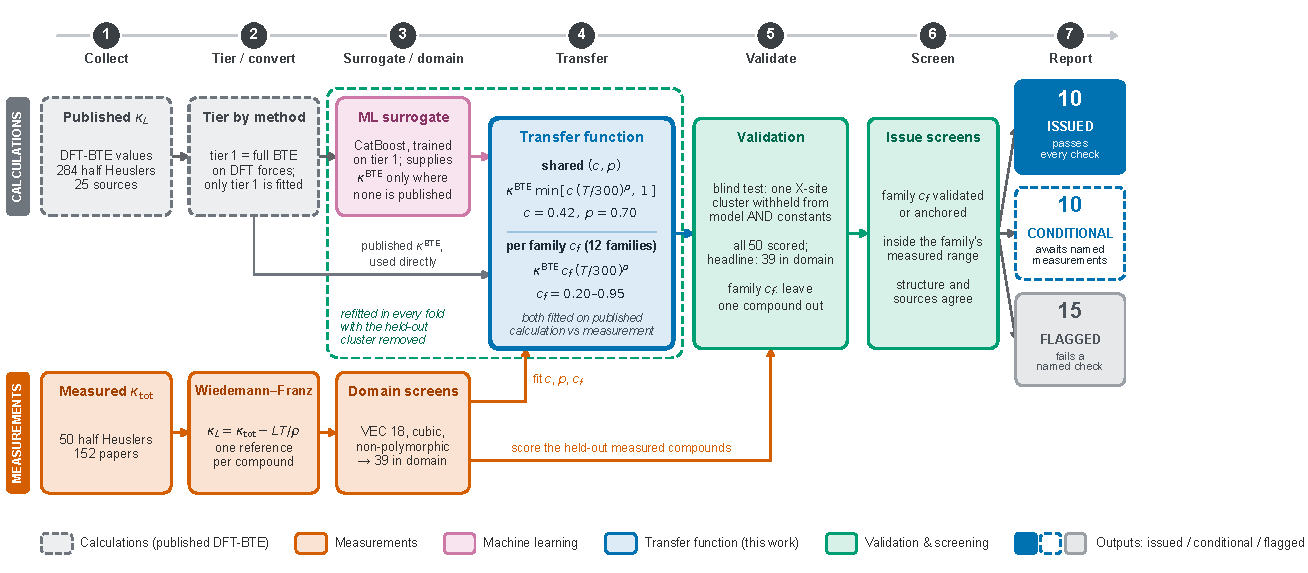
\includegraphics[width=\linewidth]{figures/fig08_method.pdf}
  \caption{\textbf{The method, end to end, in seven numbered steps.} Calculations (upper lane, grey,
  dashed) and measurements (lower lane, orange) are tiered, converted and screened separately, and
  meet only at the transfer function (blue). A published full Boltzmann-transport calculation
  (tier~1) is corrected directly; the machine-learning surrogate (pink), trained on tier~1 only,
  supplies a calculation only where none is published. The measurements fit the shared constants
  ($c$, $p$) and the per-family constants $c_f$, and separately score the held-out compounds. The
  green dashed region marks what each fold of the blind test refits with one X-site chemistry
  cluster removed. Predictions that pass the issue screens are issued; a prediction that fails a
  named check is flagged; estimates on the shared constant, in families with no usable measured
  member, are conditional.}
  \label{fig:method}
\end{figure*}

\subsection{Corpus construction}
\label{sec:dataset}

A correction from calculation to experiment can be fitted only on compounds that have both, so the
corpus records calculations and measurements separately. It holds \num{9495} temperature-resolved
values for \num{960} distinct Heusler compounds, \num{735} of them half Heuslers, and every value
records its source and how it was obtained.

Experimental values come from the Starrydata curated transport database~\cite{katsura2025starrydata},
read at its published snapshot of 1 July 2025~\cite{mato2025starrydata}, and from direct extraction
from primary publications. Starrydata aggregates curves digitised from primary publications; the
measured half-Heusler values trace to \num{152} distinct publications. For direct extraction,
multimodal large language models read the full text, tables and figures: Google Gemini
\texttt{gemini-2.5-flash} (\num{483} extractions, 4--13 July 2026) and \texttt{gemini-2.5-pro}
(\num{695} extractions, 13 July -- 18 September 2026). A retrieved record with no body text is never
passed to the model, and every extracted value must pass the physical and provenance gates below,
so no value enters the corpus on the model's authority alone. First-principles values come from
AFLOW~\cite{curtarolo2012aflow} (its AAPL transport module~\cite{plata2017an} and its AGL
Debye--Gr\"{u}neisen estimates~\cite{toher2014highthroug}, kept apart by the tiering below), the
Materials Project~\cite{jain2013commentary}, JARVIS~\cite{choudhary2020the},
OQMD~\cite{kirklin2015the} and published phonon-transport studies. Crystal structures come from the
same repositories, the Crystallography Open Database~\cite{graulis2009crystallog} and
OPTIMADE-federated sources~\cite{andersen2021optimade}.

Experiments measure the total thermal conductivity, so most measured rows separate the lattice part
by Wiedemann--Franz subtraction,
%
\begin{equation}
  \kappa_L = \kappa_\mathrm{tot} - \frac{L T}{\rho},
  \label{eq:wf}
\end{equation}
%
with the Lorenz number $L$ from the single-parabolic-band parameterisation of Kim and
Snyder~\cite{kim2015characteri}, $T$ the temperature and $\rho$ the electrical resistivity; every
row records which route produced it. Because Eq.~\eqref{eq:wf} is a difference of two measured
quantities, $\rho$ must lie in the range available to a dense intermetallic; a row outside it
reports total conductivity under a lattice label and is removed. Four further rules decide what
counts as a measurement: a value one paper quotes from another is not one; a sample digitised twice
enters once; a data deposit that republishes curves is never counted as a laboratory; and a
composition must be a Heusler. A separate gate collapses a preprint, a deposit and the article they
duplicate onto the version of record, so that one calculation is never counted as two groups. The
rules are given in full in the Extended Methods.

Figure~\ref{fig:corpus} summarises the corpus. Of the \num{735} half Heuslers with any
thermal-conductivity record, \num{284} have a full transport calculation and \num{50} have been
measured, and the evidence behind the measured set is uneven: many compounds rest on a single
publication, a few on ten or more.

\begin{figure*}[tbp]
  \centering
  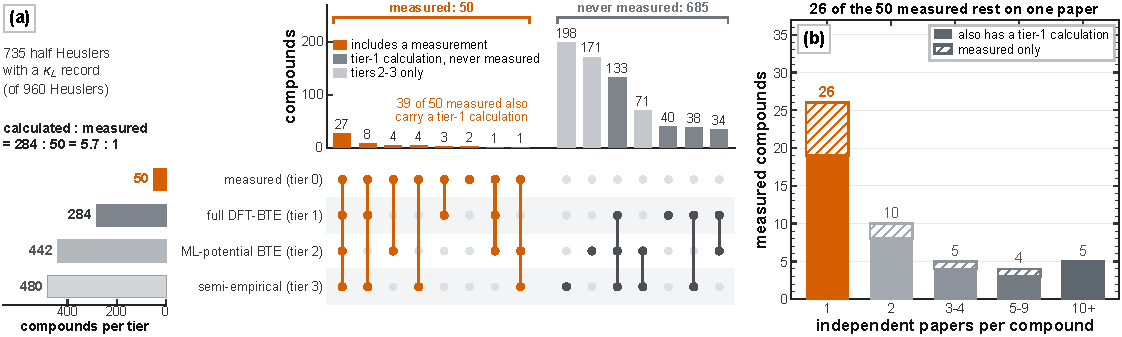
\includegraphics[width=\linewidth]{figures/fig01_corpus.pdf}
  \caption{\textbf{The half-Heusler $\kappa_L$ corpus.} (a)~The \num{735} half Heuslers with a
  thermal-conductivity record (of \num{960} Heusler compounds) by evidence type: rows are method tiers
  (measured; full DFT-BTE; ML-potential BTE; semi-empirical), columns the tier combinations
  compounds carry; column heights give compound counts and left bars tier sizes. \num{284} compounds
  carry a full calculation and \num{50} a measurement (\num{5.7}:1); \num{39} of the \num{50} also
  carry a tier-1 calculation (not the same set as the \num{39} in-domain compounds of the blind
  test). (b)~Independent publications per measured compound, a preprint and its article counted
  once; hatched, no tier-1 calculation. \num{26} of the \num{50} rest on a single publication.}
  \label{fig:corpus}
\end{figure*}

\subsection{The measured values and the choice of reference}
\label{sec:measured}

A transfer function is only as well defined as the experimental scale it maps onto. Every reference
is a stoichiometric parent compound (each coefficient within \num{0.02} of an integer), so the
doped and alloyed specimens that dominate the half-Heusler literature are excluded and the
correction measures the offset between a calculation and a measurement of the same compound. That
offset still has two sources, which we do not separate: error in the calculation itself (a
three-phonon calculation omits higher-order scattering, and the exchange-correlation functional is
approximate) and the specimen, whose point defects, grain boundaries and incomplete density are
absent from the calculation of a perfect crystal.

We never blend the curves of several laboratories, since a blend is a curve nobody measured. A fixed
ladder, reading only the specimen and the temperature coverage of each measurement and never a
calculation, chooses one reference laboratory per compound: the central laboratory when four or more
report it, otherwise the densest specimen, otherwise the widest temperature range. A
\emph{family-paper rung} makes one primary publication that measured two or more members of a family
the reference for those members, so that a family constant describes one kind of specimen. A
laboratory contradicting a consensus, a data deposit, a nanostructured specimen and a source with
fewer than four temperatures rank last but are never deleted, and a curve-shape test rejects curves
with a visibly mis-subtracted electronic term (full rules in the Extended Methods). Within the chosen
publication, the value in each \SI{100}{\kelvin} temperature bin is the median of its rows. In the
blind test, and for the compound held out in the family test, the reference is chosen without the
family-paper rung, so that it never depends on which siblings have been measured. The sources record
little about each specimen, and independent laboratories measuring the same compound disagree by a
median factor of \num{1.33}; the correction is therefore not a microstructural model but the expected
value over published practice, and every score depends on the choice of reference as well as on the
method.

\subsection{Method tiers and quality control}
\label{sec:tiering}

Every row carries a \emph{method tier}. Tier~0 is a laboratory measurement (\num{50} half Heuslers
from \num{152} publications). Tier~1 is a full solution of the phonon Boltzmann transport equation
from first-principles third-order force constants (\num{284} half Heuslers). Tier~2 is an
approximate or reduced transport route, including a transport calculation whose force constants come
from a machine-learned interatomic potential. Tier~3 is a semi-empirical or quasi-harmonic estimate:
Slack~\cite{slack1979the}, Debye--Callaway~\cite{callaway1959model} or AGL. Only tier~1 enters the
calibration and, for half Heuslers, the training of the regression model. The tier is assigned from
the method string, never from a repository's label, and tier~1 requires a positive match for a
transport solution with no disclaimer attached.

Five quality-control conditions are applied when the corpus is generated: a cubic $C1_b$ record
(space group 216) from a source that is not a prototype-substitution database; a polymorph flag for a
compound also recorded in a non-cubic space group; separation of half from full Heuslers by the site
ratio; a \SI{200}{\kelvin} temperature floor, below which a boundary-free calculation and a
boundary-limited measurement are not the same quantity; and a transport-calculation method string
for tier~1. They are stated with their reasons in the Extended Methods.

\subsection{Domain of applicability}
\label{sec:domain}

A transfer function for \emph{lattice} thermal conductivity is meaningful only where lattice
conduction dominates. The domain is half Heuslers with 18 valence electrons, a cubic $C1_b$
structure, and no other polymorph on record. Transition-metal half Heuslers are semiconducting at a
valence-electron count (VEC) of 18~\cite{graf2011simple}; away from it a large electronic term must
be removed from every measurement. VEC sums, over the three elements of the 1:1:1 formula, the group
number for groups 1--12 and the group number minus 10 for groups 13--18, with lanthanides and
actinides counted as group~3. We restrict to $\mathrm{VEC}=18$ because that is where the corpus has
support. The structural conditions follow because the calculation being calibrated is for the cubic
phase.

Two further screens apply to prediction candidates only. A candidate containing \ce{Ce}, \ce{Sm},
\ce{Eu} or \ce{Yb}, whose valence is not fixed~\cite{lawrence1981valence}, is flagged rather than
issued (the validation compound \ce{YbNiSb} is still scored), and a candidate containing a
radioactive element is excluded, since the corpus holds no training example of one.

All \num{50} measured half Heuslers are scored in the blind test; \num{44} have $\mathrm{VEC}=18$ and
\num{39} also pass the structural conditions, forming the in-domain set. The domain is defined by the
screens every candidate must pass, independently of the validation result, and the headline and its
null comparison are reported with and without the screens (Section~\ref{sec:blind}). Other
sub-populations are defined where they first appear and tabulated in the Extended Methods; figures
over different populations are not directly comparable.

\subsection{Training data, descriptors and the machine-learning model}
\label{sec:trainingdata}
\label{sec:model}

The model learns calculations, never measurements. Its label is the phonon Boltzmann-transport
conductivity of a cubic crystal,
%
\begin{equation}
  \kappa_L^{\mathrm{BTE}} \;=\; \frac{1}{3N_{\mathbf{q}}V}\sum_{\mathbf{q},s}
    C_{\mathbf{q}s}\, v_{\mathbf{q}s}^{2}\, \tau_{\mathbf{q}s},
  \label{eq:bte}
\end{equation}
%
a sum over the $N_{\mathbf{q}}$ sampled wavevectors $\mathbf{q}$ and branches $s$ of the mode heat
capacity $C_{\mathbf{q}s}$, squared group velocity $v_{\mathbf{q}s}^{2}$ and lifetime
$\tau_{\mathbf{q}s}$, divided by the cell volume $V$. The training pool holds \num{681} labels on
\num{463} compounds. Of these, \num{284} are half Heuslers (\num{230} with $\mathrm{VEC}=18$), each
labelled by a full first-principles calculation; tier-2 and tier-3 half-Heusler values are excluded.
Full Heuslers share the descriptors and enter the pool, those without a transport calculation
through a semi-empirical estimate at reduced weight; held-out scoring always uses half Heuslers
alone. Of the labels, \num{544} are at \SI{300}{\kelvin} and \num{119} at \SI{500}{\kelvin}, so the
training data constrain the temperature dependence only weakly. The labels are strongly
right-skewed, so the model is fitted on $\log_{10}\kappa_L^{\mathrm{BTE}}$; their distribution is
shown in the Extended Methods.

We train gradient-boosted decision trees (CatBoost~\cite{prokhorenkova2017catboost}). Each prediction
is the median over five random seeds. Some diagnostics are run at one seed, always seed~0, the
\emph{reference seed}, and are labelled as such; headline figures are medians over the five seeds.

\paragraph{Descriptors.} Each row is described by \num{45} descriptors of the composition, the cubic
cell and the temperature, in six groups: (i)~site properties (mass, radius and electronegativity of
X, Y and Z); (ii)~cross-site means, contrasts, spreads and ratios, including the X--Z
electronegativity difference; (iii)~Klemens-type disorder, zero throughout this stoichiometric pool
and kept only so the set is defined for substituted compositions; (iv)~cell geometry (volume per atom,
density, atoms per conventional cell, full-Heusler and quaternary flags); (v)~bond lengths from the
atomic coordinates, missing for \num{81} rows and handled natively by the model; and
(vi)~temperature, as $T$, $1000/T$ and $\log_{10}T$. The lattice parameter itself is never a
descriptor, because sources mix the primitive and conventional cells.

\subsection{Model selection}
\label{sec:modelselection}

We compared four regressors on identical rows, descriptors and weights: CatBoost, LightGBM, a
Gaussian process and kernel ridge regression, each scored out of fold on the full pool with
five-fold cross-validation grouped by element system. CatBoost has the highest $R^2$ and the lowest
RMSE and MAE (Table~\ref{tab:models}); LightGBM has the lowest median error per compound, by
\num{0.1} percentage points (pp), too small to separate the two, and we retain CatBoost. Only kernel
ridge falls clearly behind, so the results do not hinge on the choice. The comparison measures fit to
calculated labels, on element-system folds rather than the X-site clusters of the validation, and
over the whole pool, so its figures are not comparable with the half-Heusler accuracy of
Section~\ref{sec:mlrepro}. Parity plots for all four are in Section~S7 of the Supplementary
material.

\begin{table}[tbp]
  \centering
  \caption{Model selection: four regressors trained on identical rows (\num{681} rows, \num{463}
  compounds) and scored out of fold on identical element-system folds. RMSE, MAE and $R^2$ are per
  row on $\log_{10}\kappa_L$; the median error is per compound
  (Section~\ref{sec:metrics}). The retained model is in bold.}
  \label{tab:models}
  \small
  \begin{tabular}{lcccc}
    \toprule
    Regressor & RMSE & MAE & $R^2$ & median error \\
    \midrule
    \textbf{CatBoost}  & \textbf{\num{0.270}} & \textbf{\num{0.182}} & \textbf{\num{0.701}} & \SI{26.1}{\percent} \\
    LightGBM           & \num{0.273} & \num{0.186} & \num{0.695} & \SI{26.0}{\percent} \\
    Gaussian process   & \num{0.281} & \num{0.190} & \num{0.676} & \SI{26.4}{\percent} \\
    Kernel ridge       & \num{0.343} & \num{0.236} & \num{0.516} & \SI{32.3}{\percent} \\
    \bottomrule
  \end{tabular}
\end{table}

\subsection{The transfer function}
\label{sec:transfer}

A first-principles calculation describes a perfect, infinite crystal; a laboratory specimen is a
polycrystal with grain boundaries, point defects and finite density, each of which scatters phonons
the calculation lets propagate freely. For the \ce{XNiSn} half Heuslers this has been analysed directly
against measurement~\cite{schrade2017the}. The measured conductivity is therefore lower, and the
specimen contribution would be expected to grow as temperature falls and the intrinsic mean free
path grows.

\paragraph{The shared form.} We describe the offset empirically with two parameters:
%
\begin{equation}
  \kappa_L^{\mathrm{exp}}(T) \;=\; \kappa_L^{\mathrm{BTE}}(T)\;
    \min\!\left[c\left(\frac{T}{300}\right)^{p},\,1\right].
  \label{eq:transfer}
\end{equation}
%
Here $c$ sets the room-temperature reduction and $p$ its temperature dependence. The cap at one is a
modelling choice for the shared form, which keeps a calibrated value from exceeding its calculation;
it is not a physical requirement, since part of the offset is error in the calculation, which can
have either sign. The constants are fitted on published tier-1 calculations, each paired with the
reference measurement of the same compound, with no regression model involved. Such pairs exist for
\num{34} in-domain compounds (\num{429} pairs). We fit per compound,
%
\begin{equation}
  (c, p) \;=\; \operatorname*{arg\,min}_{c,\,p}\;
    \operatorname*{median}_{i \in \mathcal{C}}\;
    \operatorname*{median}_{j}
    \left|\log_{10}\frac{\hat{\kappa}(T_{ij};c,p)}{\kappa(T_{ij})}\right|,
  \label{eq:fit}
\end{equation}
%
where $\mathcal{C}$ is the set of compounds with pairs that remain after the scored compound's
\emph{held-out unit} is removed, $\hat{\kappa}$ is the corrected calculation and $\kappa$ the
reference measurement at the matched temperatures $T_{ij}$. The held-out unit is the X-site
chemistry cluster in the blind test, the bonding family in the unseen-family test, and the compound
itself in the family comparison (Section~\ref{sec:nulls}), so no scored compound informs the
constant applied to it. The error is taken in logarithm because it is multiplicative, and medians
stop a single digitisation artefact from steering the fit. On all \num{34} compounds the fit gives
the deployed $c=\num{0.42}$ and $p=\num{0.70}$; $c\,(T/300)^{p}$ then reaches one at
\SI{1036}{\kelvin}.

The magnitude is well determined and the exponent is not. Removing any one of the \num{16} chemistry
clusters among the \num{34} compounds moves $c$ within \numrange{0.41}{0.56} and $p$ within
\numrange{0.50}{0.80}; removing any one of the \num{12} bonding families moves $c$ within
\numrange{0.40}{0.54} and $p$ within \numrange{0.60}{0.80}. Over \num{200} bootstrap resamples of the
compounds, the 10th--90th percentile range is \numrange{0.35}{0.55} for $c$ but \numrange{0.45}{1.15}
for $p$. We therefore do not claim to predict the temperature dependence of an individual compound.

\paragraph{The family form.} Every bonding family with at least one member that has both a published
calculation and a usable reference measurement carries its own constant:
%
\begin{equation}
  \kappa_L^{\mathrm{exp}}(T) \;=\; \kappa_L^{\mathrm{BTE}}(T)\;
    c_f\left(\frac{T}{300}\right)^{p}, \qquad p = \num{0.70}.
  \label{eq:family}
\end{equation}
%
Twelve families qualify. Only the magnitude is refitted, by Eq.~\eqref{eq:fit} restricted to
$c_f<1$ on the family's measured members, because most families are measured over too narrow a
range to identify their own exponent. A family with two or more measured members (nine families) is
tested held out, each member predicted from the others with its own measurement withheld, and
\emph{passes}, or is \emph{validated}, only if the median error over its folds is under
\SI{25}{\percent}. A family with one member is \emph{anchored}: its figure is an in-sample fit,
never a validation. The family form carries no cap and can exceed its calculation at high
temperature, by up to \num{2.18} times, which is where the measurements of those families lie; every
issued prediction carries a factor below one.

A compound receives its family's constant wherever its family has a measured member, and the shared
constant otherwise. The leave-one-chemistry-out blind test is the exception: it is scored with the
shared constant, because a chemistry holdout leaves a compound's family-mates in training and would
not test a family constant at all.

\paragraph{Pairing a calculation with a measurement.} A calculation reported at several temperatures
is interpolated in log--log space; one reported at a single temperature is carried as
$\kappa_L^{\mathrm{BTE}} \propto 1/T$, the high-temperature limit of three-phonon Umklapp
scattering, by no more than a factor of \num{2.5} in temperature and never below
\SI{200}{\kelvin}. Independent calculations are combined by their median, and a temperature at which
they disagree by more than a factor of two is \emph{contested} and not used, for measured compounds
and candidates alike; this is why \ce{TiNiPb} is quoted at \SI{500}{\kelvin}. The full rules are in
the Extended Methods.

\paragraph{What the constants mean.} Empirical temperature dependences have been fitted to measured
half-Heusler curves before~\cite{geng2014lattice,petersen2015critical}; here we fit instead the
\emph{ratio} of measurement to calculation, and this work adds the corpus, the class-wide magnitude
and the held-out validation, not the functional form. With $\kappa_L^{\mathrm{BTE}} \propto T^{-1}$,
$p=\num{0.70}$ implies a corrected $\kappa_L \propto T^{-0.30}$. The correction is empirical, not a
boundary-scattering term: a single-boundary-length model, grey or spectral~\cite{callaway1959model},
caps the logarithmic slope of the suppression at $1-c$ (\num{0.58} at $c=\num{0.42}$), and the fitted
$p$ exceeds that cap, although its bootstrap range straddles it (derivation in the Extended Methods).
We attach no mechanism to the parameters.

\subsection{Predictions from crystal structure alone}
\label{sec:structureonly}

For a compound nobody has calculated, the model supplies $\kappa_L^{\mathrm{BTE}}$ and the transfer
function maps it onto the experimental scale. We searched DxMag~\cite{xiao2026accurate}, AFLOW, OQMD,
JARVIS and the Materials Project for cubic $C1_b$ cells inside the domain, took the lattice parameter
of the lowest-energy site ordering on record, and predicted a candidate only if its family, its X
element and every element are represented among the training half Heuslers. A prediction is graded
\emph{strong} when the model reproduces the family's own published calculations to within
\SI{25}{\percent} held out and the five seeds agree within a factor of \num{1.3}, \emph{moderate}
within \SI{50}{\percent} and \num{1.5}, and \emph{weak} otherwise. Literature status was checked in
OpenAlex~\cite{priem2022openalex}, Crossref and arXiv with a positive control; a value reported only
in a table or supplement is invisible to this search, which limits every novelty statement here. The
two steps, structure to calculation and calculation to experiment, carry errors that we report side
by side and never combine. The full procedure and two model-free cross-checks are in the Extended
Methods.

\subsection{Validation, null baselines and prediction intervals}
\label{sec:nulls}
\label{sec:intervals}

The evaluation rules for the results reported here were fixed in writing before this evaluation was
run: the definition of the shared constant and its held-out use, the single-reference rule, the
construction of the intervals at the quoted temperature, and the list of figures to be reported
whatever they showed. These documents are kept, time-stamped, in the code repository.

Every figure for the model route is obtained with the target compound's \emph{entire chemistry}
withheld: compounds are clustered by their X element and a whole cluster is removed at once
(\emph{leave-one-chemistry-out}), from the model and from the shared constant alike. Family-mates
with a different X element remain in training, so the test measures accuracy for a new X-site
substitution within a known family. There are \num{27} clusters among the \num{230} calculated
$\mathrm{VEC}=18$ half Heuslers, \num{16} among the \num{34} compounds of the published route,
\num{18} among the \num{39} in-domain compounds and \num{21} among all \num{50} measured ones. Every
threshold or model choice is made on one half of the clusters and evaluated on the other, and every
headline figure is the median over five model seeds, quoted with its range. Two \emph{null
baselines} use no compound-specific information: a constant equal to the median measured
conductivity of the training compounds, and a power law $A(T/300)^{q}$ fitted to them, both with the
same chemistry held out and the same references; the paired comparison is also made with each
cluster counted once. Family constants are tested leave-one-compound-out against the shared constant
refitted without the same compound, and the shared constant on families never measured is tested
leave-one-family-out on the \num{34} compounds of the published route.

Prediction intervals are split conformal intervals~\cite{lei2018distributi}, built from out-of-fold
residuals in logarithmic space. Each in-domain compound contributes one residual, under the
calibration it would actually receive (its family constant fitted without it, or else the shared
constant refitted without its cluster), in the temperature bin nearest the quoted temperature. For a
nominal level $\alpha$ over $m$ held-out compounds,
%
\begin{equation}
  \delta_\alpha \;=\; \Bigl\{\, \bigl|\log_{10} \rho_i \bigr| \,\Bigr\}_{(k)},
  \qquad k = \bigl\lceil (m+1)\,\alpha \bigr\rceil,
  \label{eq:conformal}
\end{equation}
%
where $\rho_i$ is the ratio of prediction to reference for compound $i$ in that bin and the band is a
factor of $10^{\delta_\alpha}$ either way. Exchangeability of the residuals is assumed, not shown,
and compounds sharing a cluster or a laboratory weaken it, so coverage is treated as a measured
frequency, evaluated leave-one-chemistry-out for each seed; the median band over seeds is deployed.
At \SI{300}{\kelvin} the bands are a factor of \num{1.62}, \num{2.56} and \num{2.85} at
\SI{50}{\percent}, \SI{80}{\percent} and \SI{90}{\percent} nominal, covering \num{20}, \num{31} and
\num{36} of the \num{39} in-domain compounds; at \SI{500}{\kelvin} they are \num{1.38}, \num{1.70}
and \num{1.89}, covering \num{20}, \num{32} and \num{36} (binomial uncertainty roughly
\SI{8}{pp}). Coverage is not validated for an anchored family or a family never measured.

\subsection{Metrics}
\label{sec:metrics}
\label{sec:definitions}

Model selection scores the fit to calculated labels \emph{per row}, on $y=\log_{10}\kappa_L$. Over
$N$ rows with labels $y_k$, out-of-fold predictions $\hat{y}_k$ and label mean $\bar{y}$,
%
\begin{gather}
  \mathrm{RMSE} = \sqrt{\frac{1}{N}\sum_{k=1}^{N}\bigl(\hat{y}_k-y_k\bigr)^2},
  \qquad
  \mathrm{MAE} = \frac{1}{N}\sum_{k=1}^{N}\bigl|\hat{y}_k-y_k\bigr|,
  \label{eq:rmse}\\
  R^2 = 1-\frac{\sum_k\bigl(\hat{y}_k-y_k\bigr)^2}{\sum_k\bigl(y_k-\bar{y}\bigr)^2};
  \label{eq:r2}
\end{gather}
%
an RMSE of \num{0.270} on the logarithm corresponds to a typical scatter by a factor of
$10^{0.270}\approx\num{1.86}$. Every other figure, including every comparison with measurement, is
reported \emph{per compound}. The error of a prediction $\hat{\kappa}$ at temperature $T$ against the
reference $\kappa$ is
%
\begin{equation}
  \mathrm{APE}(T) \;=\; \frac{\bigl|\hat{\kappa}(T) - \kappa(T)\bigr|}{\kappa(T)},
  \label{eq:ape}
\end{equation}
%
and for compound $i$ with matched temperatures $T_{ij}$,
%
\begin{equation}
  e_i \;=\; \operatorname*{median}_{j=1\ldots n_i} \mathrm{APE}(T_{ij}),
  \qquad
  r_i \;=\; \operatorname*{median}_{j} \frac{\hat{\kappa}(T_{ij})}{\kappa(T_{ij})}.
  \label{eq:err}
\end{equation}
%
We report the \emph{median error}, $\operatorname{median}_i e_i$; the fractions \emph{within a
factor of two} ($\tfrac{1}{2} \le r_i \le 2$), \emph{within \SI{30}{\percent}} ($e_i \le 0.30$) and
\emph{within \SI{25}{\percent}} ($e_i < 0.25$, the bar a family must pass); and the \emph{bias},
$\operatorname{median}_i r_i$. Aggregating per compound stops a compound measured at many
temperatures from outweighing one measured at few, and the calibration is fitted per compound for
the same reason. Differences between percentages are given in percentage points (pp).

% =============================================================================================
% SECTION 3 -- RESULTS AND DISCUSSION.
%
% Condensed 2026-10-05 (research-paper pass). Order: the offset; the transfer function (shared
% constant, family constants, Fig. fig:family (c)-(e) curves, the shared constant on families never
% measured); 2026-10-06 float pass: fig03_curves merged into fig09_family (c)-(e); fig10_ml,
% fig11_shap and fig04_blind replaced by fig15_model_blind (fig:modelblind); tab:blind moved to the
% Supplementary material; tab:famcal trimmed (spread / publications / papers -> supplement table
% tab:famsupport); tab:predictions drops the 50% column and merges basis + c_f into the family cell;
% the regression model against published calculations; what the model has learned (SHAP); the
% end-to-end blind test; the published-model check; the issued predictions; the flagged compounds
% (table and landscape figure moved to the Supplementary material); predictions from crystal
% structure alone (table folded into the prose); limits.
%
% Every number is read from data/exports/kappa_v2/paper_numbers.json or from
% data/Target_Materials/PAPER_PREDICTIONS.csv.
%   offset figure caption         offset.* (n_compounds 34, in domain: shared_constant.pairs ->
%                                 family_calibration.build_published pairs in-domain measurements)
%   curves figure + prose         curves_best3.* (n_eligible 21, eligible_median 21.7, compounds:
%                                 TiSnPt 7.7 c 0.8185 p 0.65; LuNiSb 8.0 c 0.42 p 0.70; LaBiPd 10.1
%                                 c 0.8371 p 0.65). "about 400 K" = 300 * c^(-1/p): 408 K (TiSnPt),
%                                 394 K (LaBiPd). LuNiSb two instruments: claims_ledger row
%                                 ciesielski2020thermoelec (full text read; PPMS 2-300 K, LFA 300-923 K).
%   headline without YNiBi        headline_without_YNiBi (n 38, 33.1, 24.6-35.5, 86.8, p 0.0052/0.006)
%   unscreened nulls (ref. seed)  nulls.predictors.* (36.41 / 48.67 / 48.17), nulls.paired_tests
%                                 (0.0354 / 0.0329), nulls.n_compounds 50, nulls.n_clusters 21
%   cluster-level Wilcoxon max    cluster_level_significance.wilcoxon_p_max (0.0385 / 0.0483)
%   one-parameter test            in_domain_table.one_parameter_ablation.test (Wilcoxon, ref. seed)
%   range-gate p 0.51             range_gate.p_marginal_vs_inside
%   16 of 21                      vs_published_model.ours_closer_pct 76.2 x n_common 21
%   Sb-Pt three temperatures      family_calibration.adopted.Sb-Pt.members_own.*.n_rows = 3
%   Ni-Sb blind-test members      blind_by_family.families.Ni-Sb.n = 8 (YbNiSb beside the seven)
%   HfCoAs space group 62         make_paper_predictions.structure_status (on record beside 216)
%   structure-only rows           structure_only.main_text.* (kappa_theory_300, seed spread,
%                                 kappa_exp_shared_300, family check)
% =============================================================================================

\section{Results and Discussion}
\label{sec:results}

We first measure the offset that the transfer function removes and test the transfer function on
published calculations; then the machine-learning model against published calculations; then the
two together against measurement; and finally the predictions the method issues and declines.

\subsection{Calculations exceed measurements, and the offset is regular}
\label{sec:offset}

A correction is possible only if the offset between calculation and experiment is systematic. We pair
every in-domain half Heusler that has both a published full calculation and a laboratory
measurement, each compound scored against its single reference laboratory: \num{34} compounds and
\num{429} calculation--measurement pairs, reduced for the figures to \num{189} points, one per
compound per \SI{100}{\kelvin} bin. The calculation exceeds the measurement by a median factor of
\num{1.69} (each compound's median ratio, then the median over compounds;
Fig.~\ref{fig:offset}(d)). The excess is directional, not scatter about agreement: it appears in
\num{29} of the \num{34} compounds and in \num{10} of the \num{12}
bonding families. The five exceptions, \ce{HfSnPt}, \ce{TiSnPt}, \ce{ZrSnPt}, \ce{ErBiPd}
and \ce{LaBiPd}, make up the two families whose median calculation lies below measurement,
\ce{Sn}--\ce{Pt} and \ce{Bi}--\ce{Pd}. On average the ratio of measured to calculated conductivity
rises towards one with temperature (Fig.~\ref{fig:offset}(c)), consistent with extrinsic scattering
truncating long mean free paths, although the data do not identify a mechanism.

\begin{figure*}[tbp]
  \centering
  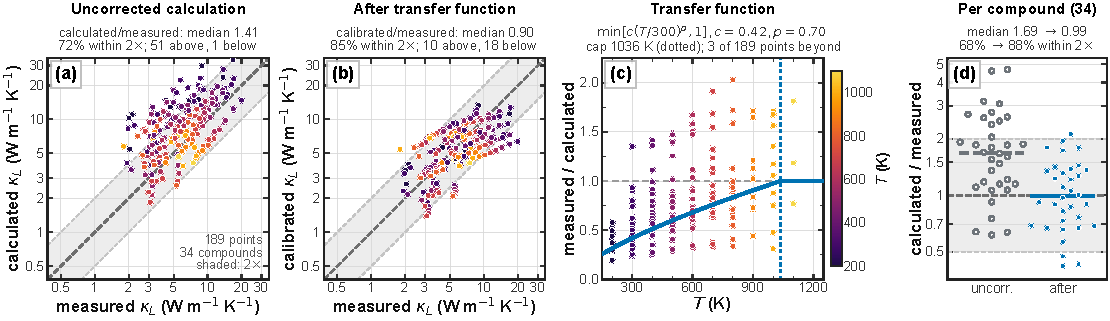
\includegraphics[width=\linewidth]{figures/fig02_offset.pdf}
  \caption{\textbf{Offset between published Boltzmann-transport calculations and measurement, and
  its removal.} (a)~Uncorrected and (b)~calibrated (Eq.~\eqref{eq:transfer}) $\kappa_L$ against
  measurement: \num{189} points, one per compound per \SI{100}{\kelvin} bin, from \num{34}
  in-domain compounds with one reference laboratory each; shaded, within a factor of two; colour,
  temperature; the statistics above (a) and (b) are per point. (c)~Measured/calculated ratio against
  $T$ with the deployed transfer function, $c=\num{0.42}$, $p=\num{0.70}$; dotted, the
  \SI{1036}{\kelvin} cap, beyond which \num{3} of the \num{189} points lie. Points above unity, where
  the calculation already lies below the measurement, are out of reach of a downward correction.
  (d)~Per-compound median calculated/measured ratio before and after correction; bars mark the
  medians (\num{1.69} $\to$ \num{0.99}; within $2\times$, \SI{68}{\percent} $\to$
  \SI{88}{\percent}), the statistics quoted in the text. Calibrated values in (b) and (d) are held
  out (shared constant refitted without each compound's chemistry cluster); the curve in (c) is the
  deployed constant, fitted on all compounds.}
  \label{fig:offset}
\end{figure*}

Correcting each compound with the shared constant refitted without its own chemistry cluster moves
the median ratio from \num{1.69} to \num{0.99} and the fraction of compounds within a factor of two
of measurement from \SI{68}{\percent} to \SI{88}{\percent} (Fig.~\ref{fig:offset}(b) and (d)). The
cap of the shared form binds only above \SI{1036}{\kelvin}, where \num{3} of the \num{189} points
lie (Fig.~\ref{fig:offset}(c)).

\subsection{The transfer function}
\label{sec:transferresults}

\paragraph{The shared constant.} Fitted on the \num{34} compounds of Section~\ref{sec:offset}, the
shared form gives $c=\num{0.42}$ and $p=\num{0.70}$. As Section~\ref{sec:transfer} shows, the
magnitude is stable under removal of any cluster or family and under a bootstrap, whereas the
exponent is not.

\paragraph{One constant per bonding family.}
\label{sec:familycal}
\label{sec:deployed}
A family \emph{member} is a compound with both a usable reference measurement and a
temperature-matched published calculation. Each of the \num{12} families with a member carries its
own constant (Eq.~\eqref{eq:family}), tested leave-one-compound-out because that is the question a
prediction poses: an unmeasured target is predicted with its measured family-mates in hand, and the
family-mates' references are re-chosen inside each fold so that a held-out compound cannot select
them.

Table~\ref{tab:famcal} and Fig.~\ref{fig:family}(a) give the families. Five are validated held out,
all within the \SI{25}{\percent} bar:
\ce{Sb}--\ce{Pt} (\SI{7.4}{\percent}), \ce{Ni}--\ce{Sb} (\SI{16.4}{\percent}), \ce{Fe}--\ce{Sb}
(\SI{17.3}{\percent}), \ce{Sn}--\ce{Pt} (\SI{21.7}{\percent}) and \ce{Co}--\ce{Sb}
(\SI{24.9}{\percent}). In \ce{Sn}--\ce{Pt} the family constant more than halves the shared
constant's error (\SI{50.4}{\percent}), and it is also clearly better in \ce{Sb}--\ce{Pt}
(\SI{30.4}{\percent} with the shared constant) and \ce{Fe}--\ce{Sb} (\SI{28.7}{\percent}). The
\ce{Sb}--\ce{Pt} figure rests on thin data: three of its four
members (\ce{DySbPt}, \ce{LuSbPt}, \ce{TbSbPt}) come from one paper at three temperatures each,
below the four-temperature rule used elsewhere. In \ce{Ni}--\ce{Sb} and \ce{Co}--\ce{Sb} the shared
constant does as well or better on the same compounds (\SI{10.1}{\percent} and
\SI{23.0}{\percent}); the pre-specified rule still gives every family with measured members its own
constant, so the issued \ce{Ni}--\ce{Sb} values carry \num{0.47} rather than the shared \num{0.42}.

\begin{table}[tbp]
  \centering
  \caption{Per-family transfer functions, $\kappa_L^{\mathrm{BTE}}\,c_f\,(T/300)^{0.70}$, with the
  shared exponent. \emph{Held out}: each member predicted from its family-mates alone, with the
  family constant and with the shared constant refitted without it (better in bold); a family is
  \emph{validated} when its held-out error is under \SI{25}{\percent}. \emph{Own paper}: the
  constant fitted on each member's own reference and scored on it, in sample, not a test.
  \textdagger, held-out test not passed; figures in Section~S14 of the Supplementary material, and
  each family's spread of member constants and its publications in Section~S15. The twelfth family,
  \ce{Sb}--\ce{Ir}, has one member that its own constant does not reproduce within the bar even in
  sample; it is listed in Section~S14. Only validated and anchored families issue predictions.}
  \label{tab:famcal}
  \footnotesize
  \setlength{\tabcolsep}{3pt}
  \begin{tabular}{lcccccl}
    \toprule
    & & & \multicolumn{2}{c}{held out (\si{\percent})} & own paper & \\
    \cmidrule(lr){4-5}
    Family & members & $c_f$ & family & shared & (\si{\percent}) & status \\
    \midrule
    \ce{Sb}--\ce{Pt} & 4 & \num{0.61} & \textbf{7.4} & 30.4 & 2.4 & validated \\
    \ce{Ni}--\ce{Sb} & 7 & \num{0.47} & 16.4 & \textbf{10.1} & 4.5 & validated \\
    \ce{Fe}--\ce{Sb} & 3 & \num{0.36} & \textbf{17.3} & 28.7 & 13.9 & validated \\
    \ce{Sn}--\ce{Pt} & 3 & \num{0.89} & \textbf{21.7} & 50.4 & 13.1 & validated \\
    \ce{Co}--\ce{Sb} & 3 & \num{0.42} & 24.9 & \textbf{23.0} & 8.2 & validated \\
    \midrule
    \ce{Bi}--\ce{Pd} & 3 & \num{0.95} & \textdagger & \textdagger & 7.3 & calibrated \\
    \ce{Ni}--\ce{Sn} & 3 & \num{0.32} & \textdagger & \textdagger & 3.0 & calibrated \\
    \ce{Co}--\ce{Sn} & 2 & \num{0.286} & \textdagger & \textdagger & 4.2 & calibrated \\
    \ce{Sb}--\ce{Pd} & 3 & \num{0.24} & \textdagger & \textdagger & 2.8 & calibrated \\
    \midrule
    \ce{Co}--\ce{Bi} & 1 & \num{0.54} & --- & --- & 6.3 & anchored \\
    \ce{Ni}--\ce{Pb} & 1 & \num{0.51} & --- & --- & 5.6 & anchored \\
    \bottomrule
  \end{tabular}
\end{table}

\begin{figure*}[tbp]
  \centering
  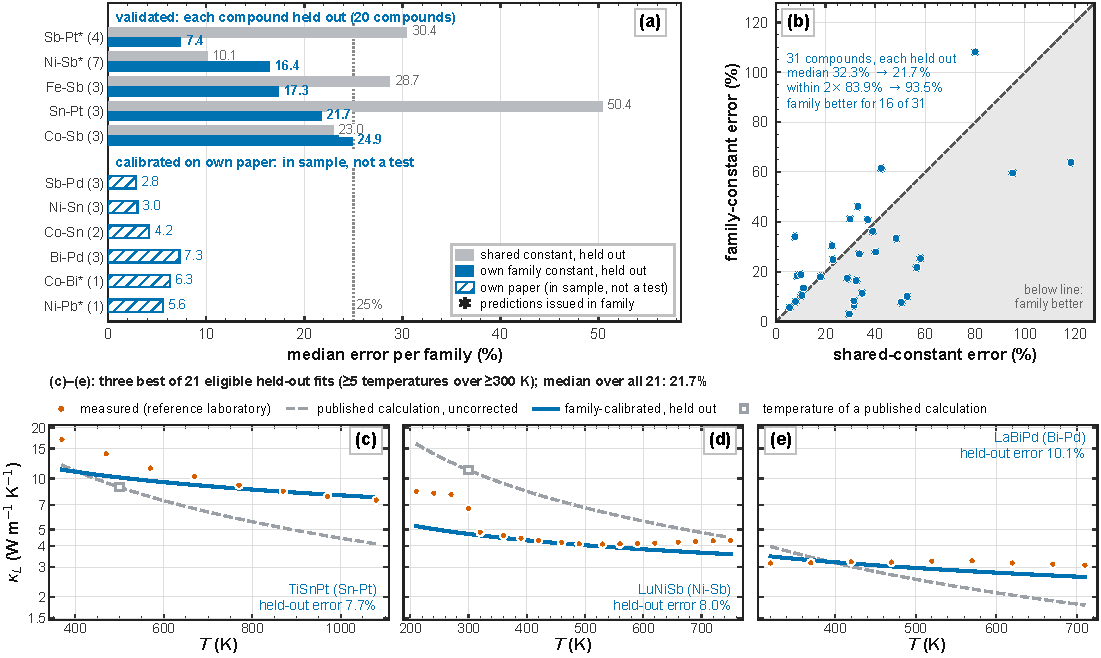
\includegraphics[width=\linewidth]{figures/fig09_family.pdf}
  \caption{\textbf{Per-family calibration on published calculations.} (a)~Median error per bonding
  family ($n$ in brackets; *, families with issued predictions). Validated families (held-out error
  below \SI{25}{\percent}): each member predicted with its family constant fitted without it (blue)
  and with the shared constant refitted without it (grey). Hatched: the four calibrated families and
  the two anchored ones, each constant fitted on its family's own reference papers and scored on
  them, in sample, not a test; held-out figures for the calibrated families are in Section~S14 of
  the Supplementary material. Dotted line, \SI{25}{\percent}. (b)~Shared- against family-constant
  error for all \num{31} held-out compounds; shaded, family constant better (better for \num{16},
  worse for \num{11}, tied for \num{4}; sign test $p=\num{0.44}$). (c)--(e)~$\kappa_L(T)$ for the
  three best of the \num{21} eligible held-out fits (at least five temperatures over at least
  \SI{300}{\kelvin}): illustrations, not a representative sample; the median over all \num{21} is
  \SI{21.7}{\percent}. Points, reference-laboratory measurement; dashed, uncorrected published
  calculation (squares at the calculated temperatures); solid, family-calibrated curve with the
  compound held out. The \ce{LuNiSb} reference joins two instruments: a steady-state measurement up
  to \SI{300}{\kelvin}, which its authors report is affected by radiative losses between
  \SI{200}{\kelvin} and \SI{300}{\kelvin}, and laser flash above~\cite{ciesielski2020thermoelec}.}
  \label{fig:family}
\end{figure*}

Every family reproduces its own reference papers closely: fitted in sample, the median error is
\SIrange{2.4}{13.9}{\percent} across the nine families, and the single-member families fit
\ce{ZrCoBi} (\ce{Co}--\ce{Bi}) to \SI{6.3}{\percent} and \ce{ZrNiPb} (\ce{Ni}--\ce{Pb}) to
\SI{5.6}{\percent}. In four families, \ce{Bi}--\ce{Pd}, \ce{Ni}--\ce{Sn}, \ce{Co}--\ce{Sn} and
\ce{Sb}--\ce{Pd}, the constant fits each paper (\SIrange{2.8}{7.3}{\percent}) but does not transfer
from one member to another within the \SI{25}{\percent} bar, because the members are different
materials as made: a nanostructured against a dense sample, or members measured in different
laboratories, as discussed below. These four are reported as calibrated, not validated; their
held-out figures and the reason in each family are in Section~S14 of the Supplementary material,
and none of them issues a prediction.

\paragraph{Pooled over the held-out compounds.} Thirty-one of the \num{34} compounds belong to a
family with at least one other measured member and can be predicted held out. On the \num{31} such
compounds the family constant gives a median error of \SI{21.7}{\percent}, with \SI{93.5}{\percent}
within a factor of two and \num{17} of the \num{31} under \SI{25}{\percent}. The shared constant,
refitted without each held-out compound and scored on the same \num{31}, gives \SI{32.3}{\percent},
with \SI{83.9}{\percent} within a factor of two. The family constant lowers the median but is not
significantly better compound by compound: it is the better of the two for \num{16} of the
\num{31}, worse for \num{11} and tied for \num{4} (two-sided sign test on the \num{27} untied,
$p=\num{0.44}$). Choosing between the capped and uncapped family forms inside each fold changes
nothing, because the uncapped form is chosen in all \num{31} folds; the capped form throughout gives
\SI{27.0}{\percent}.

Over all \num{34} in-domain compounds with a temperature-matched published calculation, the
uncorrected calculations give \SI{64.1}{\percent} median error, with \SI{70.6}{\percent} within a
factor of two. The shared constant brings that to \SI{31.9}{\percent} and \SI{85.3}{\percent}, and
the family constants to \SI{20.3}{\percent} and \SI{94.1}{\percent}. These figures follow the
protocol of the family test (all matched rows, reference chosen without the family-paper rung, shared
constant refitted without the compound itself), which is why the within-$2\times$ fractions differ
from those of Section~\ref{sec:offset} (per compound against the deployed reference, shared constant
refitted without the chemistry cluster). They also mix the \num{31} held-out compounds with the three
single-member fits, which is why we lead with the held-out comparison.

Figure~\ref{fig:family}(c)--(e) shows what a held-out family fit looks like on individual curves.
Of the \num{21} held-out compounds measured at five or more temperatures over at least
\SI{300}{\kelvin}, it shows the three with the lowest held-out family error, \ce{TiSnPt}
(\ce{Sn}--\ce{Pt}, \SI{7.7}{\percent}), \ce{LuNiSb} (\ce{Ni}--\ce{Sb}, \SI{8.0}{\percent}) and
\ce{LaBiPd} (\ce{Bi}--\ce{Pd}, \SI{10.1}{\percent}), each with its family constant fitted on its own
leave-one-out fold, exactly as the deployed route scores it; they illustrate the method at its best
and are not representative (the median over the \num{21} is \SI{21.7}{\percent}; the full
distribution is Fig.~\ref{fig:family}(b)). Because the family form is uncapped, it can raise $\kappa_L$ above the calculation: with fold constants of \num{0.82} and
\num{0.84} at $p=\num{0.65}$, the factor $c_f(T/300)^{p}$ exceeds one above about \SI{400}{\kelvin}
for \ce{TiSnPt} and \ce{LaBiPd}, so the calibrated curve rises above the uncorrected calculation
there, as the measurements do. This reproduces what the reference measurements report; it is not a
claim that the conductivity exceeds that of the perfect crystal, and every issued prediction lies
below the calculation it calibrates.

\paragraph{What a family constant describes.} Several family constants describe a single kind of
specimen (the publications behind each family are counted in Section~S15 of the Supplementary
material). All three \ce{Sn}--\ce{Pt} references come from one paper, as do three of the four in \ce{Sb}--\ce{Pt}, four of the seven in \ce{Ni}--\ce{Sb} and two
of the three in each of \ce{Bi}--\ce{Pd} and \ce{Sb}--\ce{Pd}; there the held-out test partly
measures one paper's internal consistency rather than transfer between laboratories. Two
\ce{Sb}--\ce{Pd} references are arc-melted ingots whose authors describe the transport as dominated
by grain-boundary and defect scattering~\cite{mukhopadhyay2018multifunct}. The two \ce{Co}--\ce{Sn}
members were measured on very different specimens, \ce{NbCoSn} on a near-fully dense
pellet~\cite{thiem2025thermoelec} and \ce{TaCoSn} on a heavily ball-milled nanocrystalline sample
rich in cobalt interstitials~\cite{li2019ntype}, and a constant fitted on one cannot describe the
other. An anchored family inherits its single member's specimen: \ce{ZrNiPb} was measured only on a
ball-milled sample~\cite{mao2017thermoelec}, so values issued through \ce{Ni}--\ce{Pb} describe a
milled sample, and \ce{ZrCoBi}'s reference is a \SI{98.1}{\percent} dense
pellet~\cite{zhao2018synthesis}, whereas the only other laboratory to measure it reports a value
\num{1.7} times lower near \SI{300}{\kelvin} on a far more heavily milled
specimen~\cite{zhu2018discovery}. The \ce{Co}--\ce{Bi} predictions therefore carry a wider uncertainty
than their conformal band.

\paragraph{The shared constant on families never measured.}
\label{sec:unseenfamily}
For an unmeasured family only the shared constant applies. Withholding each family in turn from the
fit and predicting its members gives, over the \num{34} compounds, a median error of
\SI{33.0}{\percent} with \SI{79.4}{\percent} within a factor of two and \SI{32.4}{\percent} within
\SI{25}{\percent}; per-family medians range from \SI{12.8}{\percent} (\ce{Ni}--\ce{Sb}) to
\SI{116.8}{\percent} (\ce{Sb}--\ce{Pd}). This calibration error travels with every shared-constant
estimate in this paper.

\subsection{The regression model reproduces published calculations}
\label{sec:mlrepro}

Where no calculation is published, the model supplies one. Scored against the published full
calculations of the \num{230} $\mathrm{VEC}=18$ half Heuslers, each predicted with its X-site
chemistry cluster withheld from training (\num{27} clusters), the median error is
\SI{21.9}{\percent} (one seed, the reference seed), with \SI{88.3}{\percent} within a factor of two
and a median ratio of \num{0.87} (Fig.~\ref{fig:modelblind}(a)). This describes only the step
from structure to calculation; the end-to-end test below already contains it, so the two errors are
never stacked. Three of the four regressors of Table~\ref{tab:models} reach nearly the same
accuracy.

\begin{figure*}[tbp]
  \centering
  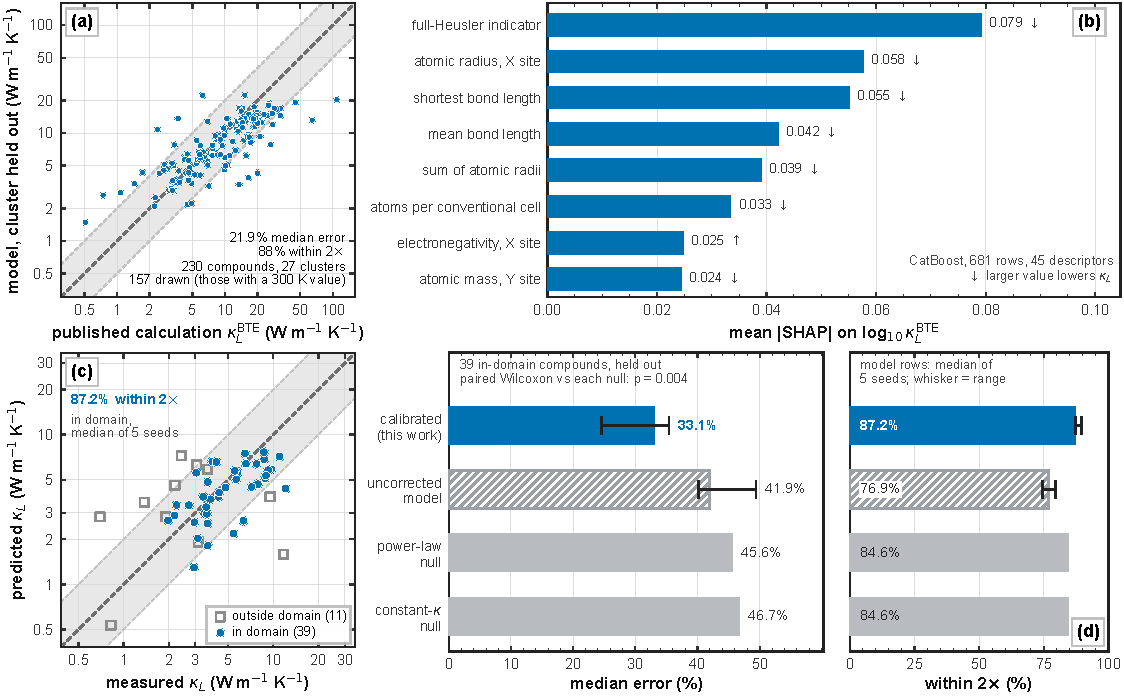
\includegraphics[width=\linewidth]{figures/fig15_model_blind.pdf}
  \caption{\textbf{From crystal structure to measured $\kappa_L$.} (a)~Model against the published
  full Boltzmann-transport calculation, each compound's X-site chemistry cluster removed from
  training: \SI{21.9}{\percent} median error and \SI{88.3}{\percent} within $2\times$ over
  \num{230} compounds (single seed; per compound over all calculated temperatures); those with a
  \SI{300}{\kelvin} value are drawn. Shaded, within a factor of two. (b)~The eight descriptors with
  the largest mean $|\textsc{shap}|$ attribution to $\log_{10}\kappa_L^{\mathrm{BTE}}$; arrows give
  the direction of the effect of a larger value. The training pool includes full Heuslers, so the
  full-Heusler indicator, which ranks first, partly reflects the make-up of the pool; the full
  attribution is in Section~S7 of the Supplementary material. (c)~Blind test against measurement, the chemistry
  cluster held out of both the model and the transfer function: filled, the \num{39} compounds
  inside the domain of applicability; open, the \num{11} outside it. Points are from the reference
  seed; the printed within-$2\times$ fraction is the five-seed median. (d)~Median error and fraction
  within $2\times$ on the \num{39} in-domain compounds for the calibrated route, the uncorrected
  model, and the power-law and constant-$\kappa$ nulls, both nulls fitted with the chemistry held
  out; model rows are the median of five seeds with the seed range as whiskers, the nulls are
  seed-free; paired Wilcoxon $p=\num{0.004}$ against each null.}
  \label{fig:modelblind}
\end{figure*}

\subsection{What the model has learned}
\label{sec:shap}

We decompose the reference-seed model, fitted on all \num{681} training rows, with \textsc{shap}
(SHapley Additive exPlanations)~\cite{lundberg2017a}, which assigns each descriptor an additive
contribution to each prediction; on the $\log_{10}$ target a contribution of $+0.1$ multiplies the
predicted calculation by about \num{1.26}. Figure~\ref{fig:modelblind}(b) shows the eight
descriptors with the largest mean absolute contribution, and Section~S7 of the Supplementary
material the twelve largest with the contribution to every training row; signs are read from the
correlation between a descriptor's value and its contribution (in parentheses: mean
$|\textsc{shap}|$, then that correlation). The full-Heusler flag leads (\num{0.079}, \num{-0.99}): a full Heusler is predicted to conduct less. Size
and bond length come next: the X-site radius (\num{0.058}), the shortest bond (\num{0.055}), the
mean bond length (\num{0.042}) and the sum of radii (\num{0.039}) all lower the prediction as they
grow (correlations \num{-0.71} to \num{-0.93}), as do more atoms per conventional cell (\num{0.033},
\num{-0.98}) and a heavier Y site (\num{0.024}, \num{-0.82}). The X-site electronegativity
(\num{0.025}, \num{+0.43}) and $1/T$ (\num{0.018}, \num{+0.90}) raise it. This is consistent with
phonon physics: heavier atoms, longer and softer bonds and more atoms per cell lower a lattice's
conductivity, and Umklapp scattering weakens as temperature falls. Consistency does not show that the
model has learned that physics.

Three cautions apply. The attribution explains the model of the \emph{calculation}, not of a
measurement, which also depends on the specimen. Correlated descriptors share attribution (the sum
of radii and the mean radius, the shortest and mean bond lengths, atoms per cell and the
full-Heusler flag; correlation map in Section~S7 of the Supplementary material), so the ranking describes groups
of descriptors more reliably than individual ones. And the full-Heusler flag partly reflects the
make-up of the pool, whose full-Heusler labels include semi-empirical estimates; it shifts all
half-Heusler predictions together and does not reorder them.

\subsection{End to end: from crystal structure to measurement}
\label{sec:blind}

This is the paper's central accuracy figure: how close the full chain, model plus shared transfer
function, comes to measurement for a compound whose chemistry was withheld from every fitted step.
We score the \num{39} in-domain half Heuslers, each against its single reference laboratory with its
X-site chemistry cluster removed from both the model's training and the fit of the shared constant.

The calibrated prediction has a median error of \SI{33.1}{\percent} and places \SI{87.2}{\percent} of
compounds within a factor of two of measurement (Fig.~\ref{fig:modelblind}(c) and (d)), both
medians over five model seeds; the full table, with the fraction within \SI{30}{\percent} and the
bias of every route, is in Section~S16 of the Supplementary material. Across seeds the median error
ranges from \SI{24.6}{\percent} to \SI{35.4}{\percent}, so it should be read as roughly one third; the within-$2\times$ fraction (\SIrange{87.2}{89.7}{\percent})
and the rank correlation are stable by comparison. Without the correction the same model output gives
\SI{41.9}{\percent} and \SI{76.9}{\percent}; the correction moves the median ratio of predicted to
measured conductivity from \num{1.40} to \num{0.90}. The \num{39} include \ce{YNiBi}, whose every
measured curve fails the curve-shape test (its lattice conductivity rises with temperature) and which
keeps its measurement, ranked last, so that the scored population does not depend on that test.
Without \ce{YNiBi} the headline is \SI{33.1}{\percent} (seed range \SIrange{24.6}{35.5}{\percent})
over \num{38} compounds, with \SI{86.8}{\percent} within a factor of two, and the paired comparison
with the null baselines gives $p=\num{0.005}$ and $p=\num{0.006}$ (medians over seeds).

\paragraph{Against compound-blind baselines.}
\label{sec:vsnulls}
The constant and power-law null baselines, refitted with the same chemistry held out and scored
against the same references, give \SI{46.7}{\percent} and \SI{45.6}{\percent} median error, against
our \SI{33.1}{\percent} (Fig.~\ref{fig:modelblind}(d)). A paired Wilcoxon signed-rank test on the per-compound
errors gives $p=\num{0.004}$ against each null at the median over seeds, and $p$ is below \num{0.05}
against both on every seed. Compounds of one chemistry cluster share a model fold and often a
laboratory, so we repeat the test counting each of the \num{18} clusters once, by its median error:
the cluster-level Wilcoxon test gives $p<0.05$ on every seed against both nulls (largest \num{0.039}
against the constant and \num{0.048} against the power law), but the cluster-level sign test is not
significant on every seed ($p$ from \num{0.0013} to \num{0.48} against the constant and from
\num{0.0013} to \num{0.096} against the power law). With two nulls, five seeds and no correction for
multiple comparisons, the cluster-level evidence is marginal. Both nulls place slightly fewer
compounds within a factor of two (\SI{84.6}{\percent}), so the gain lies in the typical error rather
than in the tail.

\paragraph{Without the domain screens.} Over all \num{50} measured half Heuslers the same protocol
gives \SI{38.6}{\percent} median error (seed range \SIrange{36.8}{38.8}{\percent}), with
\SI{78.9}{\percent} within a factor of two, against \SI{47.3}{\percent} uncorrected. The comparison
with the nulls holds, more weakly: at the reference seed, over the \num{50} compounds (\num{21}
clusters), the model route gives \SI{36.4}{\percent} against \SI{48.7}{\percent} for the constant null
and \SI{48.2}{\percent} for the power law (paired Wilcoxon $p=\num{0.035}$ and $p=\num{0.033}$).

\paragraph{Outside the domain.}
\label{sec:failure}
The eleven compounds the screens exclude (\ce{AlNiSb}, \ce{BaAgSb}, \ce{LaSbPd}, \ce{LiAlGe},
\ce{LiAlSi}, \ce{LiZnSb}, \ce{MgAgSb}, \ce{MgNiSb}, \ce{NbCoSb}, \ce{VCoSb}, \ce{VNiSn}) behave as a
separate population: at the reference seed their median error is \SI{86.4}{\percent}, against
\SI{31.7}{\percent} inside the domain (Mann--Whitney $p=\num{5.1e-5}$), with \SI{36.4}{\percent}
within a factor of two and a median bias of \num{1.74} (open squares in
Fig.~\ref{fig:modelblind}(c)).

\paragraph{Ranking, temperature term and semi-empirical estimates.} Spearman's $\rho$ between
predicted and measured conductivity is \num{0.662} (seed range \numrange{0.642}{0.699}); at a fixed
temperature this ordering comes from the model, and the correction adds the temperature term and the
absolute scale of a screening threshold. Without the temperature term
($\kappa_L^{\mathrm{exp}} = c\,\kappa_L^{\mathrm{BTE}}$) the error rises to \SI{38.5}{\percent} and
the within-$2\times$ fraction falls to \SI{82.1}{\percent}; at the reference seed (one seed) the
paired difference is \num{7.7} pp (Wilcoxon $p=\num{0.0143}$), the two-parameter form closer for
\SI{61.5}{\percent} of compounds. Published Slack~\cite{slack1979the} and Debye--Callaway estimates,
on the \num{22} in-domain compounds that have one, give \SI{91.6}{\percent} with
\SI{54.5}{\percent} within a factor of two and a bias of \num{1.92}; they are published values with
no holdout and are not paired with the blind-test set.

\paragraph{Where the error falls, and a family-informed baseline.}
\label{sec:familynull}
At the reference seed the worst families on the model route are \ce{Co}--\ce{Sn}
(\SI{59.4}{\percent}) and \ce{Ni}--\ce{Sn} (\SI{55.4}{\percent}), three compounds each, while
\ce{Ni}--\ce{Sb} (eight compounds: the seven members of Table~\ref{tab:famcal} and \ce{YbNiSb}) is at
\SI{13.7}{\percent}; this grouping is descriptive, since the holdout unit is the X site. A stronger
baseline fits a power law to the measured $\kappa(T)$ of the held-out compound's own family, with no
calculation. On the \num{34} in-domain compounds where it is defined (the \num{39} minus \ce{AlVNi},
\ce{YNiBi}, \ce{ZrCoBi}, \ce{ZrNiPb} and \ce{ZrSbIr}; not the \num{34} of the published route), it
gives \SI{25.4}{\percent} against \SI{31.6}{\percent} for the model route at the reference seed, with
neither significantly better (paired Wilcoxon $p=\num{0.99}$; model closer for \SI{50.0}{\percent}).
Where a family has been measured we do not beat it on absolute accuracy, but it cannot order
compounds within a family or say anything where no member is measured. For scale, calibrating a
published calculation with the shared constant gives \SI{32.3}{\percent} on the \num{31} compounds of
the family test, comparable to the model route's \SI{33.1}{\percent} on a different population.

\subsection{A published machine-learned model}
\label{sec:sdnnff}

Elemental-SDNNFF obtains $\kappa_L$ through the Boltzmann transport equation on a neural-network
force field~\cite{rodriguez2023millionsca}, so its values are tier~2 and were never labels; the same
paper's ShengBTE values are tier~1 and enter the published-calculation median for \num{6} of the
\num{18} compounds below (\ce{NbFeSb}, \ce{TaFeSb}, \ce{TiNiSn}, \ce{VFeSb}, \ce{ZrCoSb},
\ce{ZrNiSn}). On those \num{18} in-domain compounds SDNNFF reproduces the published calculations at
\SI{300}{\kelvin} to a median \SI{18.8}{\percent} (ratio \num{0.99}). Against measurement, on the
\num{21} in-domain compounds it covers, it lies a median factor of \num{2.01} above the reference
(\SI{101.4}{\percent} median error, \SI{42.9}{\percent} within a factor of two), and the published
calculations lie a factor of \num{1.99} above measurement on their \num{18} (a different set from
Section~\ref{sec:offset}, at \SI{300}{\kelvin} only, for matching windows from \SI{\pm 25}{\kelvin}
to \SI{\pm 100}{\kelvin}): the offset arrives intact at the end of a screening pipeline. The shared
constant, refitted without each compound's chemistry cluster, brings the SDNNFF values to
\SI{36.8}{\percent} with \SI{76.2}{\percent} within a factor of two (paired Wilcoxon $p=\num{0.0033}$),
so the correction transfers to an independent source of calculations. Our model route gives
\SI{44.7}{\percent} on the same \num{21} (reference seed, \SI{71.4}{\percent} within a factor of two),
closer to measurement than raw SDNNFF for \num{16} of the \num{21} (paired Wilcoxon
$p=\num{0.0055}$) but not as close as calibrated SDNNFF, in a comparison tilted towards SDNNFF, whose
values are given no holdout.

\subsection{Predictions for unmeasured compounds}
\label{sec:screening}
\label{sec:issued}

We apply the family route to half Heuslers that have a published transport calculation but no
measurement. A candidate is issued only if it meets every condition below:
\begin{enumerate}
  \item \textbf{Inside the domain of applicability} (Section~\ref{sec:domain}), with no radioactive
        and no valence-fluctuating element.
  \item \textbf{A bonding family whose constant has been checked}: \emph{validated} (held-out error
        under \SI{25}{\percent}) or \emph{anchored} on a single member whose in-sample fit is under
        the same bar, an anchored prediction carrying that label (Table~\ref{tab:famcal}).
  \item \textbf{A full transport calculation}, independent calculations agreeing within a factor of
        two at the quoted temperature.
  \item \textbf{Inside, or only marginally outside, the family's measured range.} A value beyond the
        family's measured span by less than a factor of \num{1.33}, the median disagreement between
        laboratories, is issued with a \emph{marginal} label; a value further outside is flagged.
\end{enumerate}

Ten compounds meet every condition (Table~\ref{tab:predictions}, Fig.~\ref{fig:predictions}). Three
lie inside the span of a validated family: \ce{TmSbPt} in \ce{Sb}--\ce{Pt}, and \ce{GdNiSb} and
\ce{TbNiSb} in \ce{Ni}--\ce{Sb}, each differing from the measured members only on the rare-earth
site. Three are marginal extrapolations in \ce{Sb}--\ce{Pt}: \ce{ErSbPt} and \ce{HoSbPt} a factor of
\num{1.15} and \num{1.12} above the family's span, and \ce{GdSbPt} \num{1.03} below it. As a check,
the \num{6} measured compounds lying this close outside their family-mates' span were predicted held
out to a median of \SI{17.4}{\percent}, \num{3} of them under \SI{25}{\percent}, against
\SI{18.8}{\percent} for the \num{19} inside it (two-sided Mann--Whitney $p=\num{0.51}$). Four issue
through anchored families: \ce{HfCoBi} and \ce{TiCoBi} through \ce{Co}--\ce{Bi}, and \ce{HfNiPb} and
\ce{TiNiPb} through \ce{Ni}--\ce{Pb}. Four of the ten issue through \ce{Sb}--\ce{Pt}, whose
validation rests mainly on one paper (Section~\ref{sec:familycal}). \ce{TiCoBi}, \ce{HfNiPb} and \ce{TiNiPb} are quoted at
\SI{500}{\kelvin}, the temperature of their only uncontested calculation (for \ce{TiNiPb}, the two
\SI{300}{\kelvin} calculations disagree \num{5.6}-fold).

\begin{table*}[tbp]
  \centering
  \caption{The ten issued predictions of lattice thermal conductivity for half Heuslers with a
  published transport calculation and no measurement, each through its own family's constant
  (Table~\ref{tab:famcal}). $T$ is \SI{300}{\kelvin}, or \SI{500}{\kelvin} where that is the
  temperature of the only uncontested calculation; $\kappa_L^{\mathrm{BTE}}$ is the median published
  calculation at $T$. The \SI{90}{\percent} intervals are conformal at the quoted temperature; the
  \SI{50}{\percent} intervals, a factor of \num{1.62} (\SI{300}{\kelvin}) or \num{1.38}
  (\SI{500}{\kelvin}) either way, are drawn in Fig.~\ref{fig:predictions}. For the anchored families
  their coverage is not validated. Span places the value relative to the range of the family's
  compounds measured near \SI{300}{\kelvin}: inside it, or beyond it by the factor shown (marginal).
  An anchored family defines no span.}
  \label{tab:predictions}
  \small
  \begin{tabular}{llccccc}
    \toprule
    Compound & Family (basis, $c_f$) & $T$ & $\kappa_L^{\mathrm{BTE}}$ & \textbf{Predicted} &
      \SI{90}{\percent} interval & span \\
    & & (\si{\kelvin}) & \multicolumn{3}{c}{(\si{\watt\per\meter\per\kelvin})} & \\
    \midrule
    \ce{TmSbPt} & \ce{Sb}--\ce{Pt} (validated, \num{0.61}) & 300 & 5.86 & \textbf{3.57} & 1.25--10.17 & inside \\
    \ce{GdNiSb} & \ce{Ni}--\ce{Sb} (validated, \num{0.47}) & 300 & 8.38 & \textbf{3.94} & 1.38--11.23 & inside \\
    \ce{TbNiSb} & \ce{Ni}--\ce{Sb} (validated, \num{0.47}) & 300 & 9.59 & \textbf{4.51} & 1.58--12.85 & inside \\
    \ce{ErSbPt} & \ce{Sb}--\ce{Pt} (validated, \num{0.61}) & 300 & 7.18 & \textbf{4.38} & 1.54--12.48 & \num{1.15} above \\
    \ce{HoSbPt} & \ce{Sb}--\ce{Pt} (validated, \num{0.61}) & 300 & 7.00 & \textbf{4.27} & 1.50--12.17 & \num{1.12} above \\
    \ce{GdSbPt} & \ce{Sb}--\ce{Pt} (validated, \num{0.61}) & 300 & 3.34 & \textbf{2.04} & 0.72--5.81 & \num{1.03} below \\
    \midrule
    \ce{HfCoBi} & \ce{Co}--\ce{Bi} (anchored, \num{0.54}) & 300 & 18.60 & \textbf{10.04} & 3.52--28.61 & --- \\
    \ce{TiCoBi} & \ce{Co}--\ce{Bi} (anchored, \num{0.54}) & 500 & 19.10 & \textbf{14.75} & 7.80--27.88 & --- \\
    \ce{HfNiPb} & \ce{Ni}--\ce{Pb} (anchored, \num{0.51}) & 500 & 9.96 & \textbf{7.26} & 3.84--13.72 & --- \\
    \ce{TiNiPb} & \ce{Ni}--\ce{Pb} (anchored, \num{0.51}) & 500 & 13.91 & \textbf{10.14} & 5.37--19.16 & --- \\
    \bottomrule
  \end{tabular}
\end{table*}

% [!t]: at [tbp] the figure plus caption exceeds \topfraction and LaTeX set it alone on a float
% column with half the column empty; ! lifts the fraction limits so it heads the column instead.
\begin{figure}[!t]
  \centering
  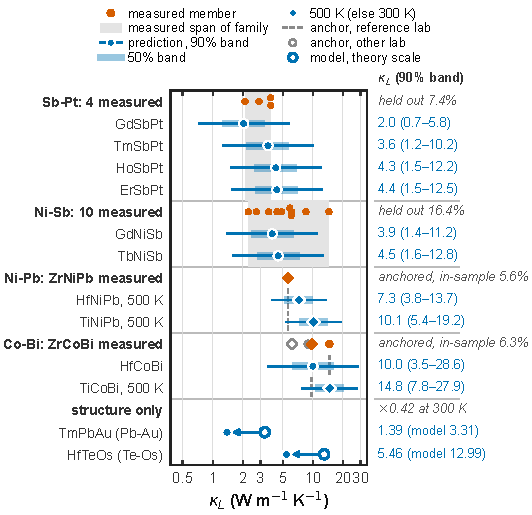
\includegraphics[width=\columnwidth]{figures/fig05_predictions.pdf}
  \caption{\textbf{Issued predictions beside the measurements that license them.} Each row is one
  issued compound at its quoted temperature (diamonds, \SI{500}{\kelvin}; otherwise
  \SI{300}{\kelvin}), with its \SI{50}{\percent} (thick) and \SI{90}{\percent} (thin) conformal
  intervals. Validated families: orange dots, measured members near \SI{300}{\kelvin}; grey band, the
  span they define. A family's measured count includes compounds without a published calculation,
  so it can exceed its member count in Table~\ref{tab:famcal}. Anchored families (one measured
  member): orange marker and dashed line, that member's reference-laboratory value at the quoted
  temperature; open grey marker, a second laboratory's. Bottom: the two structure-only predictions,
  the model's calculation-scale value (open) and the value after the shared transfer function
  (filled). The model error (Fig.~\ref{fig:modelblind}(a)) and the transfer-function error
  (Section~\ref{sec:unseenfamily}) are reported separately, not combined.}
  \label{fig:predictions}
\end{figure}

The conformal bands (Section~\ref{sec:intervals}) are a factor of \num{1.62} and \num{2.85} at
\SI{300}{\kelvin} (per-seed ranges \numrange{1.61}{1.67} and \numrange{2.70}{3.02}) and \num{1.38}
and \num{1.89} at \SI{500}{\kelvin} (\numrange{1.31}{1.41} and \numrange{1.86}{1.94}) for the
\SI{50}{\percent} and \SI{90}{\percent} levels. The calculations being calibrated come from published
high-throughput
studies~\cite{li2025highthroug,ohnishi2026database,miyazaki2021machine,carrete2014finding,trans2022lattice},
most from one~\cite{miyazaki2021machine}. Seven of the ten rest on a single published calculation at
the quoted temperature. Independent calculations of the same half Heusler disagree by a median
factor of \num{1.37}, and the band describes the error of the transfer function, not the spread among
its inputs, so where only one calculation exists the band is a lower bound on the uncertainty. Nine
of the ten rest on a calculation at a single temperature (\ce{HfCoBi} on two), so no other
temperature is quoted. \ce{GdNiSb} also carries a structural caveat the databases do not record: it
has been reported in a high-temperature \ce{AlB2}-type hexagonal form beside the low-temperature
\ce{MgAgAs}-type cubic one~\cite{skolozdra1997magnetic}, and the prediction is for the cubic phase.

\subsection{Flagged compounds, and what would release them}
\label{sec:refusals}

Fifteen compounds carry a calibrated value but are declined (\emph{flagged}); Section~S13 of the
Supplementary material tabulates each with the check it fails and draws every status on one axis. Nine are
\ce{Bi}--\ce{Pd} compounds, a family calibrated on its papers but not validated held out; seven also
lie a factor of \numrange{1.36}{1.86} above the \SIrange{3.2}{3.5}{\watt\per\meter\per\kelvin} span
of the two \ce{Bi}--\ce{Pd} compounds measured near room temperature. \ce{TmSbPd} and \ce{DySbPd}
belong to \ce{Sb}--\ce{Pd}, likewise calibrated but not validated, and \ce{DySbPd} is also
polymorphic. \ce{LaSbPt} and \ce{ScSbPt} are clear extrapolations in a validated family, a factor of
\num{2.00} below the measured \ce{Sb}--\ce{Pt} floor and \num{1.97} above its ceiling. \ce{HfSbIr}
and \ce{TiSbIr} belong to \ce{Sb}--\ce{Ir}, whose single measured member its own constant does not
reproduce within the bar. The range gate is a conservative
choice rather than a validated filter: the two held-out compounds that lay further outside their
family's span were predicted to a median of \SI{18.4}{\percent}, but two cases cannot justify issuing
clear extrapolations.

Ten further estimates, in \ce{Ni}--\ce{Bi}, are conditional. The family's only measured member,
\ce{YNiBi}, reports a lattice conductivity that rises with temperature, which its authors attribute
to a bipolar contribution~\cite{li2015synthesis}, so the family cannot be calibrated. On the shared
constant the ten lie at \SIrange{2.21}{4.95}{\watt\per\meter\per\kelvin} at \SI{300}{\kelvin};
Section~S1 of the Supplementary material lists them with the two measurements that would release
them, and one of them,
\ce{SmNiBi}, is also flagged because samarium's valence is not fixed. Across the three statuses the
conformal band has the same relative width; what changes is the evidence behind the value, not its
stated precision.

Not every gap can be closed by a measurement. The cobalt arsenides \ce{XCoAs} (X = Ti, Zr, Hf) have
published calculations but no measured family member, and the two synthesised, \ce{ZrCoAs} and
\ce{HfCoAs}, form the orthorhombic \ce{Co2Si} type~\cite{kleinke1998crystal}. The polymorph screen
catches \ce{HfCoAs}, which has an orthorhombic record (space group 62), but not \ce{ZrCoAs} or
\ce{TiCoAs}, whose records carry only the cubic cell.

\subsection{Predictions from crystal structure alone}
\label{sec:structonly}

For compounds with no published lattice-thermal-conductivity calculation, the model supplies
$\kappa_L^{\mathrm{BTE}}$ and the shared constant maps it onto the experimental scale. Each value
carries two separately validated errors, which we state side by side rather than combine: the model
step, \SI{21.9}{\percent} median error (one seed) with \SI{88.3}{\percent} within a factor of two
against published calculations (Section~\ref{sec:mlrepro}), and the calibration step, the shared
constant on a family never measured, \SI{33.0}{\percent} median with \SI{79.4}{\percent} within a
factor of two (Section~\ref{sec:unseenfamily}). Two compounds are graded strong on the evidence for
their model step; Fig.~\ref{fig:predictions} (bottom) gives both values for each. No conformal band is
given, because its coverage is not validated for a family never measured.

\ce{TmPbAu} (\ce{Pb}--\ce{Au}; OQMD cubic cell, $a=\SI{6.782}{\angstrom}$, the lowest-energy
ordering). The six \ce{Pb}--\ce{Au} half Heuslers with published calculations are reproduced held out
to between \SI{1}{\percent} and \SI{13}{\percent} (median \SI{8.6}{\percent}), and the seeds agree
within a factor of \num{1.11}. The model gives \SI{3.31}{\watt\per\meter\per\kelvin} and the shared
constant ($c=\num{0.42}$) \SI{1.39}{\watt\per\meter\per\kelvin} at \SI{300}{\kelvin}. We found no
published report of \ce{TmPbAu}; a family neighbour, \ce{TbAuPb}, has been grown as single crystals in
the cubic half-Heusler structure~\cite{agarwal2026thermodyna}.

\ce{HfTeOs} (\ce{Te}--\ce{Os}; AFLOW cubic cell, $a=\SI{6.33}{\angstrom}$, the lowest-energy
ordering). The strong grade rests on one member, \ce{TiTeOs}, reproduced to \SI{0.5}{\percent} held
out; the seeds spread by a factor of \num{1.23}. The model gives \SI{12.99}{\watt\per\meter\per\kelvin}
and the shared constant \SI{5.46}{\watt\per\meter\per\kelvin}. The SDNNFF value for the twin
\ce{ZrTeOs}~\cite{rodriguez2023millionsca}, carried to hafnium by the twin ratio of the Extended
Methods, gives \SI{14.06}{\watt\per\meter\per\kelvin}, of which the model value is \num{0.92}; that
ratio was validated on calculated pairs (\SI{12.2}{\percent} against \SI{9.8}{\percent} for the
model), not on a machine-learned input, so the cross-check is weaker than its validation suggests. We
found no published report of \ce{HfTeOs}.

The search also found further compounds with no published $\kappa_L$ and a group with only a
machine-learned value from a published screen; Section~S11 of the Supplementary material reports
them, together with two compounds in calibrated families that are flagged.

\subsection{Limits of the method}
\label{sec:limitations}

\textbf{Temperature dependence is not predicted.} One exponent serves every compound and it is
poorly determined (bootstrap range \numrange{0.45}{1.15} against \numrange{0.35}{0.55} for $c$;
Section~\ref{sec:transfer}), and the training labels sit mostly at \SI{300}{\kelvin}. Every value in
this paper is a value at a stated temperature, and none should be read as a curve.

\textbf{One reference laboratory per compound.} Laboratories measuring the same in-domain compound
disagree by a median factor of \num{1.33} over all pairs of measurements (\num{1.36} taking each
compound's median), so an error of a third is close to the reproducibility of the field, and per-family
errors may fall below that level partly because each compound is scored against one chosen reference.

\textbf{The compounds are not independent.} They share chemistry clusters, bonding families and, in
places, a laboratory, so the effective sample is smaller than \num{39}; the cluster-level tests
address the first, not the shared laboratories.

\textbf{A family constant is interpolation within the family}, and in several families the
family-mates are one paper's specimens. A family nobody has measured receives only the shared
constant, with its \SI{33.0}{\percent} median error, and the capped shared correction cannot raise a
calculation that already lies below its measurement.

\textbf{The issued values rest on few calculations.} Seven of the ten rest on a single published
calculation at the quoted temperature, and most on one study. A systematic error there would pass
undiluted into those values; a transfer function calibrates the scale of a calculation, not its
correctness.

\textbf{Training is restricted to full calculations}, leaving \num{284} half Heuslers to learn from.
The pool still contains two compounds that are not Heuslers, \ce{BaBrCl} and \ce{NaAgO}, and
\num{81} rows without bond descriptors; the model handles a missing descriptor natively, and the
effect on the reported accuracy is expected to be small.

\textbf{Structure-only values carry two errors and assume a structure}: neither compound has, as far
as we could find, been synthesised, so each value is conditional on the cubic phase forming.

\textbf{Alternatives tested.} A correction without the temperature term (Section~\ref{sec:blind}), a
capped family form, a two-stage (hurdle) model, a magnitude-dependent calibration term, and training
on experimental or doped-composition values were tested and not adopted, because they did not
improve held-out accuracy consistently.

% =============================================================================================
% SECTION 4 -- CONCLUSIONS.
%
% Condensed 2026-10-05 (research-paper pass). Shape: the pair and what each step does; the
% end-to-end result with its nulls and the unscreened figure; the family constants (passing the
% 25% bar and beating the shared constant kept apart); what the method delivers; its limits; the
% measurements that would most improve it.
%
% Numbers from data/exports/kappa_v2/paper_numbers.json:
%   1.69 / 10 of 12               offset.median_ratio_calc_over_meas, families_with_median_ratio_above_1
%   21.9                          ml_generator_validation.median_ape (single seed)
%   33.1 / 87.2 / 39              in_domain_table.seed_medians.calibrated, .n
%   41.9                          in_domain_table.seed_medians.uncorrected_surrogate
%   46.7 / 45.6                   in_domain_table.nulls
%   0.048, sign test              cluster_level_significance.wilcoxon_p_max.power (0.0483); .sign_p_range
%   33.1 / 86.8 / 38 / 0.005, 0.006   headline_without_YNiBi
%   38.6 / 78.9 / 50              headline.unconditional, blind_test.compounds
%   36.4 vs 48.7 / 48.2, p 0.035 / 0.033   nulls.predictors, nulls.paired_tests (reference seed)
%   32.3 / 31                     deployed_route.held_out.global_on_same_compounds, .n
%   101.4 -> 36.8                 vs_published_model.sdnnff_median_ape / .sdnnff_calibrated_median_ape
%   5 of 9; shared better in 3    family_calibration.adopted.*.loo_family_ape vs .loo_global_ape
%   21.7, 16 / 11 / 4, 0.44       deployed_route.held_out
%   10 / 15 / 7 / 10 conditional  predictions.counts, predictions.issued_single_calculation_source,
%                                 conditional.n
%   1.39 / 5.46; 33.0             structure_only.main_text.*; shared_constant_unseen_family.median_ape
%   0.35-0.55, 0.45-1.15          calibration.stability.bootstrap c / p (p10-p90)
%   1.33                          source_disagreement.laboratories.median_factor
% =============================================================================================

\section{Conclusions}
\label{sec:conclusions}

Used as a pair, machine learning and transfer-function calibration predict the measured lattice
thermal conductivity of half Heuslers from crystal structure. The machine-learned model reproduces
published first-principles calculations to a median error of \SI{21.9}{\percent} (one seed) with each
chemistry cluster held out, and what it has learned is consistent with phonon physics. The transfer
function is needed because the calculations run high, by a median factor of \num{1.69} and in
\num{10} of \num{12} bonding families, and it can be closed-form because that offset is regular.

Holding each compound's chemistry cluster out of both steps, inside a domain of applicability fixed
by the screens every candidate must pass, the median error is \SI{33.1}{\percent} and
\SI{87.2}{\percent} of \num{39} compounds lie within a factor of two, against \SI{41.9}{\percent}
uncorrected and \SI{46.7}{\percent} and \SI{45.6}{\percent} for constant and power-law null baselines.
The improvement is significant per compound on every model seed; counting each cluster once, the
Wilcoxon test gives $p < 0.05$ on every seed (largest \num{0.048}) but the cluster-level sign test is
not significant on every seed, so the cluster-level evidence is marginal. Without \ce{YNiBi}, whose
measured curve is flagged (Section~S3 of the Supplementary material), the figures are \SI{33.1}{\percent}
and \SI{86.8}{\percent} of \num{38} ($p = \num{0.005}$ and \num{0.006}). Without the domain screens,
over all \num{50} measured compounds, they are \SI{38.6}{\percent} and \SI{78.9}{\percent}, and at the
reference seed the unscreened route still improves on both nulls (\SI{36.4}{\percent} against
\SI{48.7}{\percent} and \SI{48.2}{\percent}; $p = \num{0.035}$ and \num{0.033}). The route performs
comparably to calibrating a published calculation (\SI{32.3}{\percent} on the \num{31} compounds of
the family test, a different set), and the correction carries over to an independent machine-learned
force field, lowering its median error against measurement from \SI{101.4}{\percent} to
\SI{36.8}{\percent}.

A magnitude refitted per bonding family is validated held out in five families, at
\SIrange{7.4}{24.9}{\percent}; in two of them (\ce{Co}--\ce{Sb} and \ce{Ni}--\ce{Sb}) the shared
constant does as well or better on the same compounds, and the family constant is applied there by
the pre-specified rule. Four further families are calibrated on their own papers but do not transfer
between members held out, because their members are different materials as made; they issue no
prediction. The best figure, \ce{Sb}--\ce{Pt} at
\SI{7.4}{\percent}, rests on one paper's three members at three temperatures each. Pooled, the family
constant lowers the median error from \SI{32.3}{\percent} to \SI{21.7}{\percent}, but it is better for
\num{16} compounds, worse for \num{11} and tied for \num{4} (sign test $p = \num{0.44}$), so it is not
significantly better compound by compound.

We issue \num{10} predictions with intervals, flag \num{15} candidates with the reason named for each,
and report \num{10} estimates as conditional on a measurement in their family. From crystal structure
alone we give $\kappa_L$ at \SI{300}{\kelvin} of \SI{1.39}{\watt\per\meter\per\kelvin} for
\ce{TmPbAu} and \SI{5.46}{\watt\per\meter\per\kelvin} for \ce{HfTeOs}, compounds for which we find no
published report; each carries, uncombined, the model's \SI{21.9}{\percent} and the shared constant's
\SI{33.0}{\percent} on families never measured.

The method estimates $\kappa_L$ at a stated temperature but does not predict its temperature
dependence: over a bootstrap of compounds the magnitude stays between \num{0.35} and \num{0.55} while
the exponent ranges from \num{0.45} to \num{1.15}. Scores depend on the single reference laboratory
chosen per compound, in a field whose laboratories disagree by a median factor of \num{1.33}, and the
compounds share clusters, families and laboratories. A family constant interpolates within its
family, three families rest on a single measured compound, and the intervals are validated only on
in-domain compounds. Seven of the ten issued predictions rest on a single calculation source at the
quoted temperature. The method should not be used outside its domain.

A single synthesis and measurement of the cubic phase can falsify any issued prediction. The
measurements that would most improve the method are a first measurement in a family with no measured
member, such as \ce{Pb}--\ce{Au} or \ce{Te}--\ce{Os}; a second, bulk member from another laboratory in
each family that rests on one compound or one paper; wide-range measurements on dense specimens to
constrain the exponent; and two sound \ce{Ni}--\ce{Bi} measurements, free of the bipolar contribution
that rules out the existing \ce{YNiBi} curve, which would release nine of the ten conditional
estimates. For this class the binding constraint is experimental: what the conditional estimates lack
is a measured member of their family, not a calculation.


\section*{Data availability}
\label{sec:data-availability}

% Counts: provenance_sources.* (189 measurement / 188 in the reference list / 1 with no bib entry;
% 29 calculation / 26 in the reference list) and corpus.source_dois_behind_measured (152),
% corpus.half_measured_tier0 (50), in data/exports/kappa_v2/paper_numbers.json. The removed-row
% records are the release_data/audit/ files copied by build_release_data.py (AUDIT_GLOBS).
The following are archived at \repourl:
\begin{itemize}[itemsep=1pt, topsep=3pt, leftmargin=1.5em]
  \item the prediction lists: for every candidate, the calculated and calibrated values, the quoted
        temperature, the prediction intervals, the status (issued, flagged or conditional on a
        measurement) and the reason for that status;
  \item the predictions from crystal structure alone, with the source of each structure;
  \item the fitted transfer-function constants, the per-compound blind-test scores and the output
        of every model seed;
  \item a record of every row that a data-quality rule removed from the corpus or moved to a
        different method tier, each with the rule responsible;
  \item the code that rebuilds the corpus from its sources and generates every figure and number in
        this paper.
\end{itemize}
Candidate structures were taken from public databases (DxMag, AFLOW, OQMD, JARVIS and the Materials
Project). We do not redistribute bulk copies of those databases or of Starrydata. The Starrydata
snapshot used is cited~\cite{mato2025starrydata}, so that the corpus can be regenerated exactly.

The measurements analysed here are not ours. Across the whole corpus they come from \num{189}
publications, \num{152} of which lie behind the \num{50} measured half Heuslers. The transport
calculations come from \num{29} publications. The supplementary material cites every calculation
source and every measurement source but one, so the provenance claim of
Section~\ref{sec:dataset} can be checked rather than taken on trust. We list them there, not here,
only because they would otherwise outnumber the works this paper discusses. The one uncited
measurement source has a digital object identifier (DOI), \texttt{10.36410/jcpr.2020.21.3.319},
that is registered with neither Crossref nor DataCite, so it cannot be resolved into a reference.
Every measured row of the corpus carries the DOI of the work it came from; calculated rows drawn
from public databases carry a source URL instead, because those repositories are not identified by
DOI.

% CRediT (Contributor Roles Taxonomy). Elsevier asks for this, and it is the modern answer to the
% ambiguity of author order: it states who did what, so nobody has to infer contribution from
% position in the list. Roles below are drawn from the standard fourteen-term taxonomy -- adjust
% them to what each author actually did, and have each author confirm their own line.
\section*{CRediT authorship contribution statement}

\textbf{Shivam Randive:} Conceptualization, Methodology, Software, Formal analysis,
Data curation, Investigation, Validation, Writing -- original draft.
\textbf{Heet Lungaria:} \heetroles
\textbf{Ojaswini Randive:} Visualization, Writing -- review \& editing.
\textbf{Himanshu Pandey:} Supervision, Resources, Project administration,
Writing -- review \& editing.

\section*{Funding}

This research did not receive any specific grant from funding agencies in the public, commercial,
or not-for-profit sectors.

\section*{Declaration of competing interest}

The authors declare that they have no known competing financial interests or personal relationships
that could have appeared to influence the work reported in this paper.

% Elsevier requires this as a NAMED statement placed after the competing-interest declaration and
% before the reference list, under the heading below (policy revised October 2025). An AI tool is
% never an author. Use of AI in the RESEARCH belongs in the Methods as well, which is why the
% Gemini extraction is also described in Section~\ref{sec:dataset}. Extraction counts and dates are
% those of the extraction database (data/heusler.sqlite, extractions table, status 'ok'); the Claude
% model is the one used in the 2026-10 analysis and drafting sessions.
\section*{Declaration of generative AI and AI-assisted technologies in the manuscript preparation process}

Corpus values were extracted from primary publications with Google Gemini models:
\texttt{gemini-2.5-flash} (483 extractions, 4--13 July 2026) and \texttt{gemini-2.5-pro}
(695 extractions, 13 July -- 18 September 2026). Every extracted value had to pass the physical
and provenance gates described in Section~\ref{sec:dataset}, and no value entered the corpus on a
model's authority alone. Claude Opus 5.5 (Anthropic) was used to write and audit the analysis and
plotting code, including the code that generates every figure, and to assist in drafting the
manuscript text. The authors reviewed all code and text, edited
them as needed, and take full responsibility for the content of the published article.

\section*{Acknowledgements}

\acknowledgementtext

\bibliographystyle{elsarticle-num}
\bibliography{references}

\end{document}
